  \documentclass[a4paper,12pt]{article}

% Pacotes necessários
\usepackage[utf8]{inputenc}
\usepackage[T1]{fontenc}
\usepackage[portuguese]{babel}
\usepackage{graphicx}
\usepackage[a4paper,margin=1in]{geometry} % Configuração de margens
\usepackage{float}

% Título
\title{\textbf{Leis de Ohm e Kirchhoff (Amperímetro)}}
\author{
    Arthur Silva de Vasconcelos \and Carlos Eduardo de Lima \and Italo Santos
}
\date{11 de janeiro de 2025}

\begin{document}

\maketitle
\begin{center}
    \textbf{Professor Orientador: Claudio Lenz Cesar} \\
    \textbf{Instituição: IMPATech}
\end{center}
\vspace{1cm}

\section{Lei de Ohm}
\subsection{Introdução}
\leavevmode

Este experimento tem como objetivo explorar a relação entre tensão, corrente e resistência em um circuito elétrico, verificando a proporcionalidade entre essas grandezas conforme previsto pela Lei de Ohm. A partir de medições realizadas em diferentes pontos do circuito, será possível determinar a corrente elétrica, avaliar o comportamento do sistema e calibrar os resistores utilizados.  

Além de confirmar a teoria, o experimento aborda aspectos práticos, como a influência das incertezas nas medições e a precisão dos componentes envolvidos. Essa abordagem permite compreender limitações reais de instrumentos e dispositivos, destacando a relevância da experimentação no estudo de fenômenos elétricos e na validação de conceitos teóricos.  

Com isso, este trabalho reforça a aplicação prática da Lei de Ohm, oferecendo uma base para o entendimento dos princípios fundamentais da eletricidade e para o desenvolvimento de habilidades analíticas na interpretação de resultados experimentais.

\subsection{Montagem}
\leavevmode

Antes de toda montagem do experimento físico, foi realizada uma simulação no ambiente virtual do TinkerCad do nosso circuito, EXPLICAÇÃO DA MONTAGEM. Ademais, fizemos uso do código (.ino) do Voltimetro disponibilizado pelo professor para extrair os dados do circuito.

\vspace{1em}

\begin{figure}[H]
    \centering
    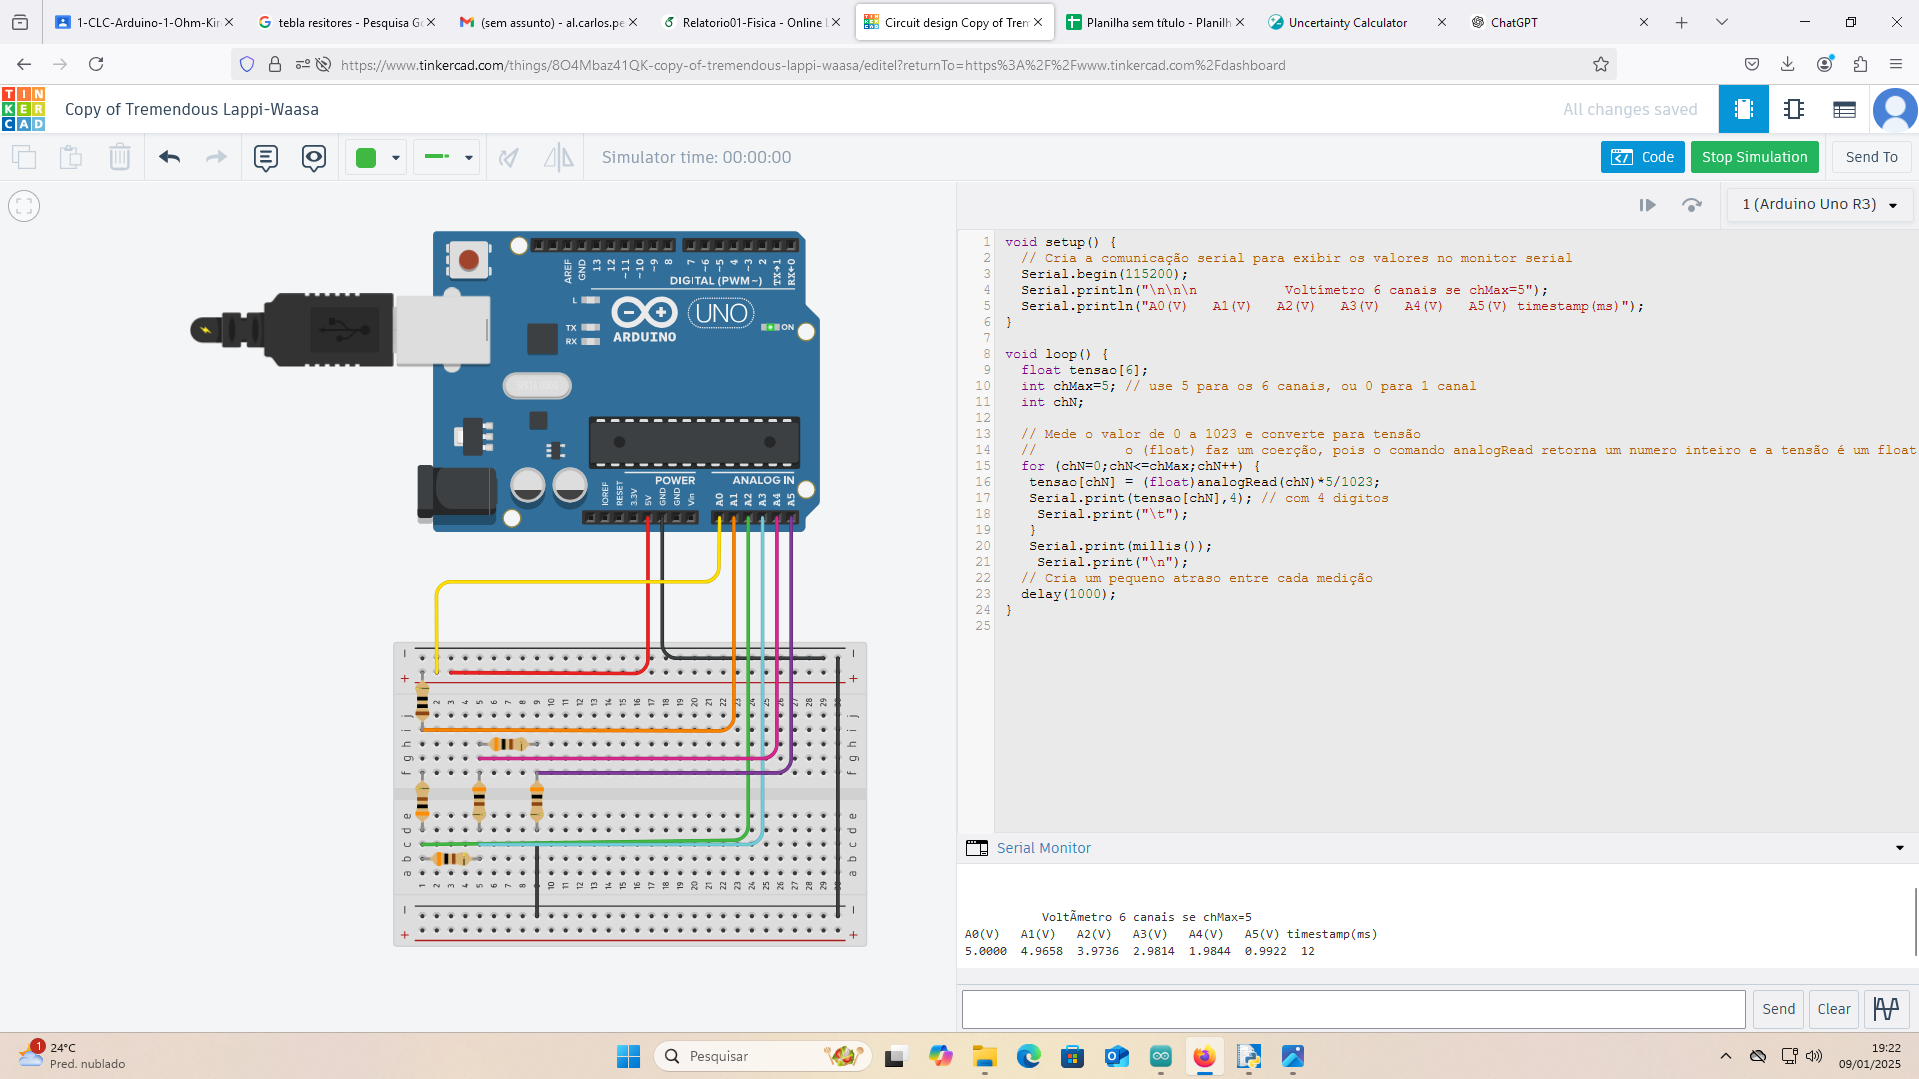
\includegraphics[width=0.8\textwidth]{Captura de tela 2025-01-09 192301.png} % Substitua pelo nome do arquivo da imagem
    \caption{Simulação do circuito no TinkerCad.}
    \label{fig:tinkercad}
\end{figure}

\vspace{1em}

Logo após essa simulação no TinkerCad, reproduzimos o circuito no Arduino Uno para comparação dos dados obtidos.

\vspace{1em}

\begin{figure}[H]
    \centering
    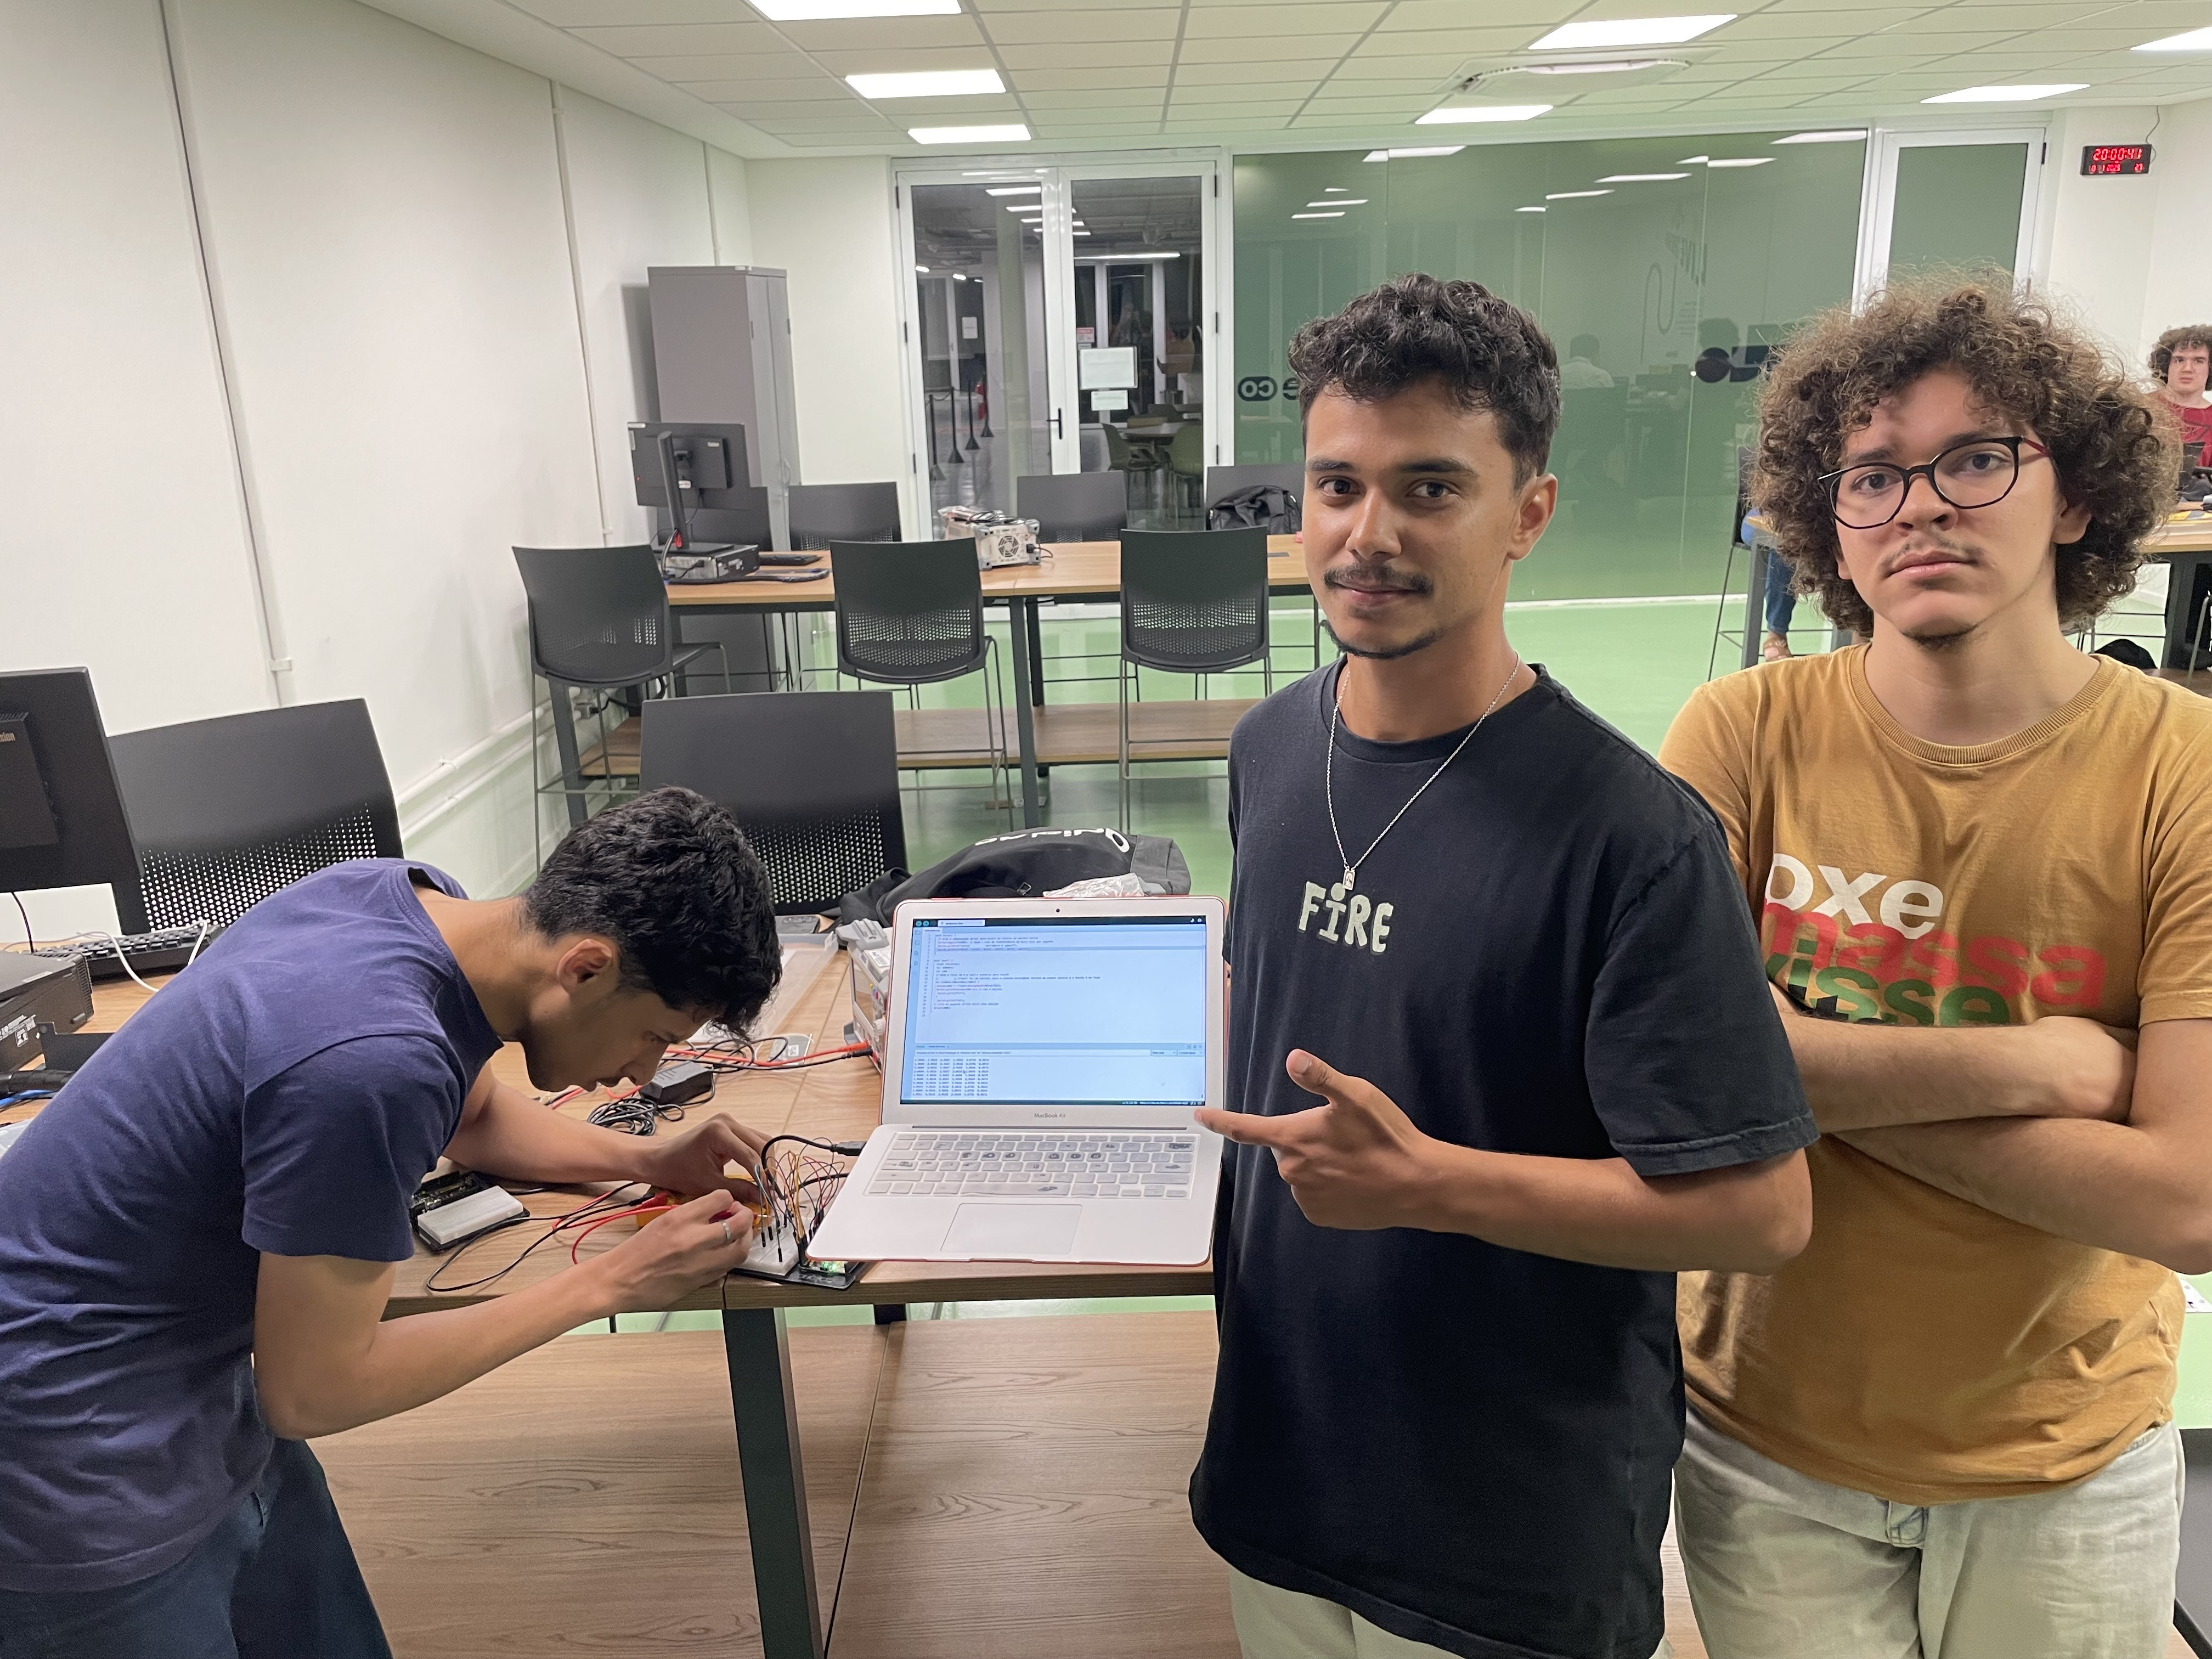
\includegraphics[width=0.8\textwidth]{IMG_1113.jpeg} % Substitua pelo nome do arquivo da imagem
    \caption{Montagem do experimento pelos integrantes do grupo.}
    \label{fig:arduino}
\end{figure}

\vspace{1em}


\begin{figure}[H]
    \centering
    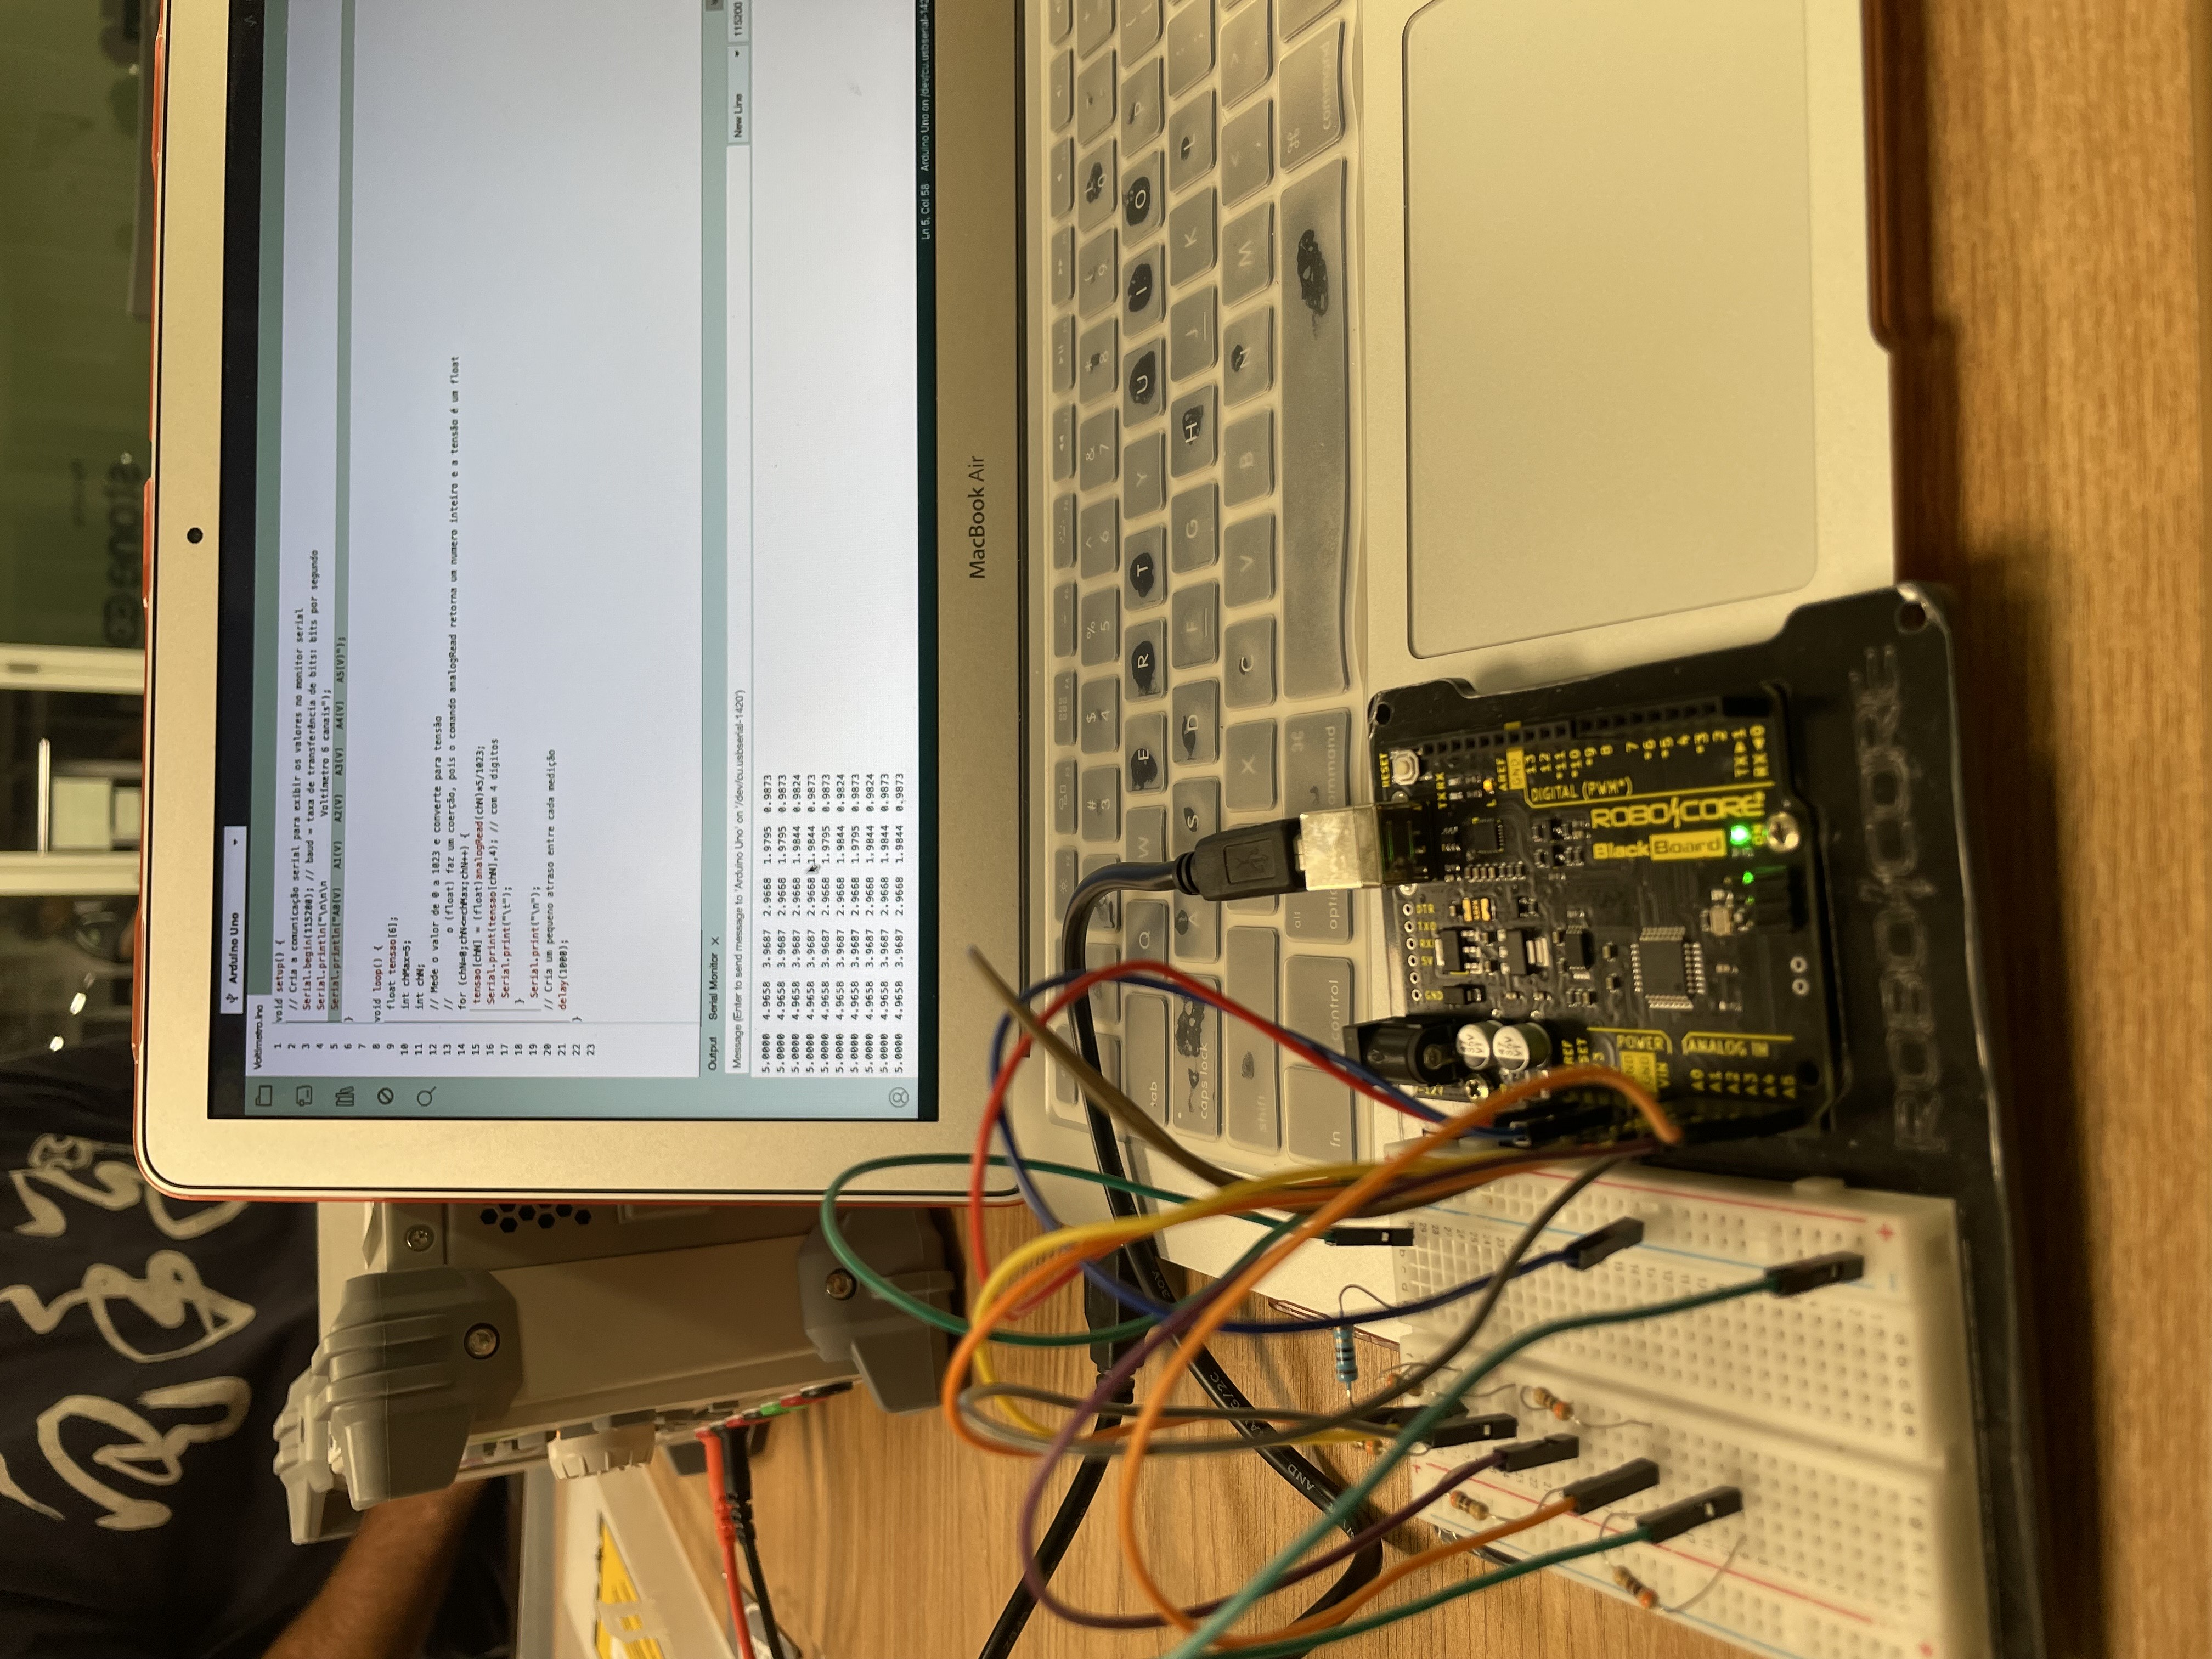
\includegraphics[width=0.8\textwidth]{IMG_1111.jpeg} % Substitua pelo nome do arquivo da imagem
    \caption{Circuito montado no Arduino Uno.}
    \label{fig:arduino}
\end{figure}

\vspace{1em}

\subsection{Resultados}
\subsubsection{Dados}
\leavevmode

Depois de toda a simulação e a realização do experimento no Arduino Uno, obtivemos os seguintes valores das tensões em A0 até A5:

\vspace{1em}

\begin{figure}[H]
    \centering
    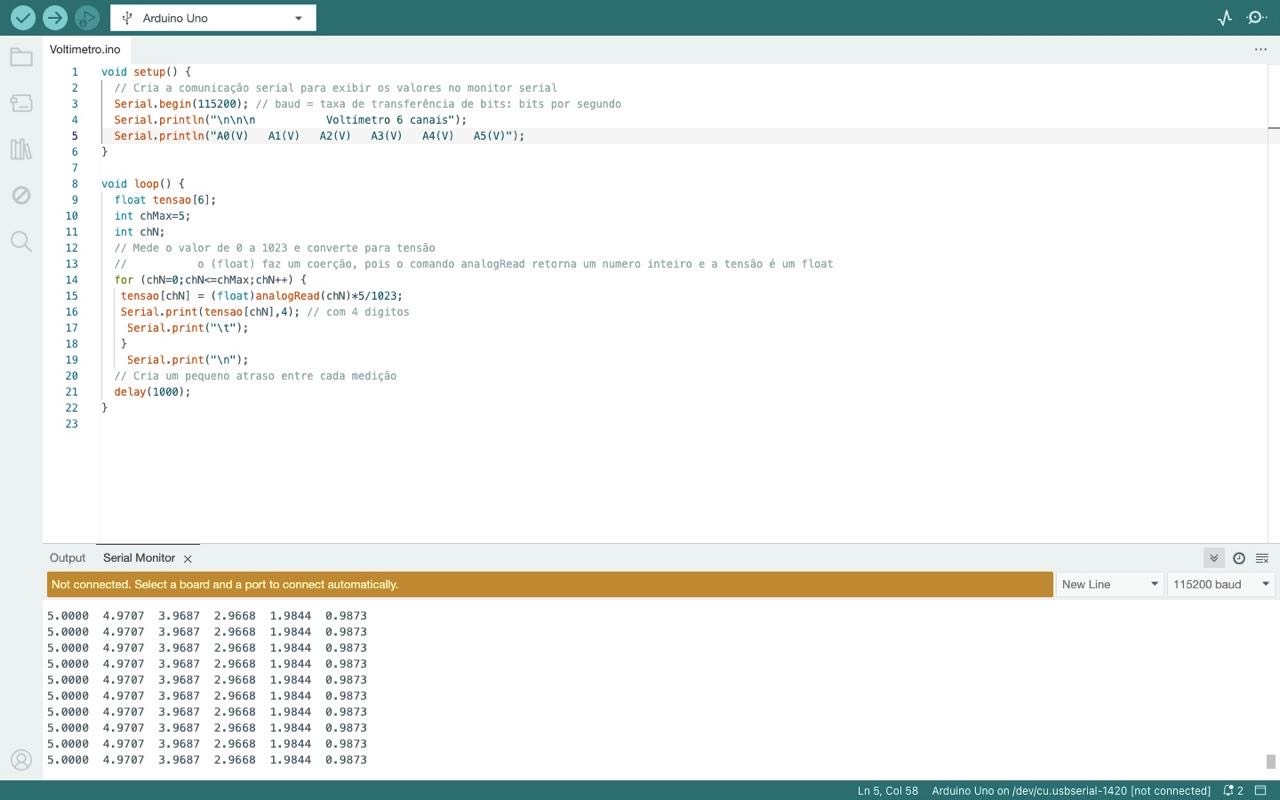
\includegraphics[width=0.8\textwidth]{14afe182-753e-4c66-8e25-b3968096270d.jpeg} % Substitua pelo nome do arquivo da imagem
    \caption{Tensões Obtidas.}
    \label{fig:arduino}
\end{figure}

\vspace{1em}
\begin{table}[ht]
    \centering
    \begin{tabular}{|c|c|}
        \hline
        Pino do Arduino & Tensão (V) \\
        \hline
        A0 & 5.000 ± 0.005 \\
        A1 & 4.970 ± 0.005 \\
        A2 & 3.968 ± 0.005 \\
        A3 & 2.966 ± 0.005 \\
        A4 & 1.984 ± 0.005 \\
        A5 & 0.987 ± 0.005 \\
        \hline
    \end{tabular}
    \caption{Tabela de tensões medidas nos pinos A0 a A5.}
    \label{tab:tensoes}
\end{table}

\begin{itemize}
    \item Para a tensão, o erro mínimo é dado pela resolução do ADC do Arduino ($10 \, \text{bits}$):
    \[
    \Delta V = \frac{5 \, \text{V}}{1023} \approx 0.0049 \, \text{V}.
    \]
\end{itemize}

\vspace{1em}

\subsubsection{Gráfico V x R e Calibração dos resistores de 300 \(\Omega\)}
\leavevmode

Com todas as tensões obtidas, podemos retirar alguns resultados desses dados. Para isso, foi criado um código em Python para a plotagem dos gráficos e realização dos cálculos.

\vspace{1em}

\begin{figure}[H]
    \centering
    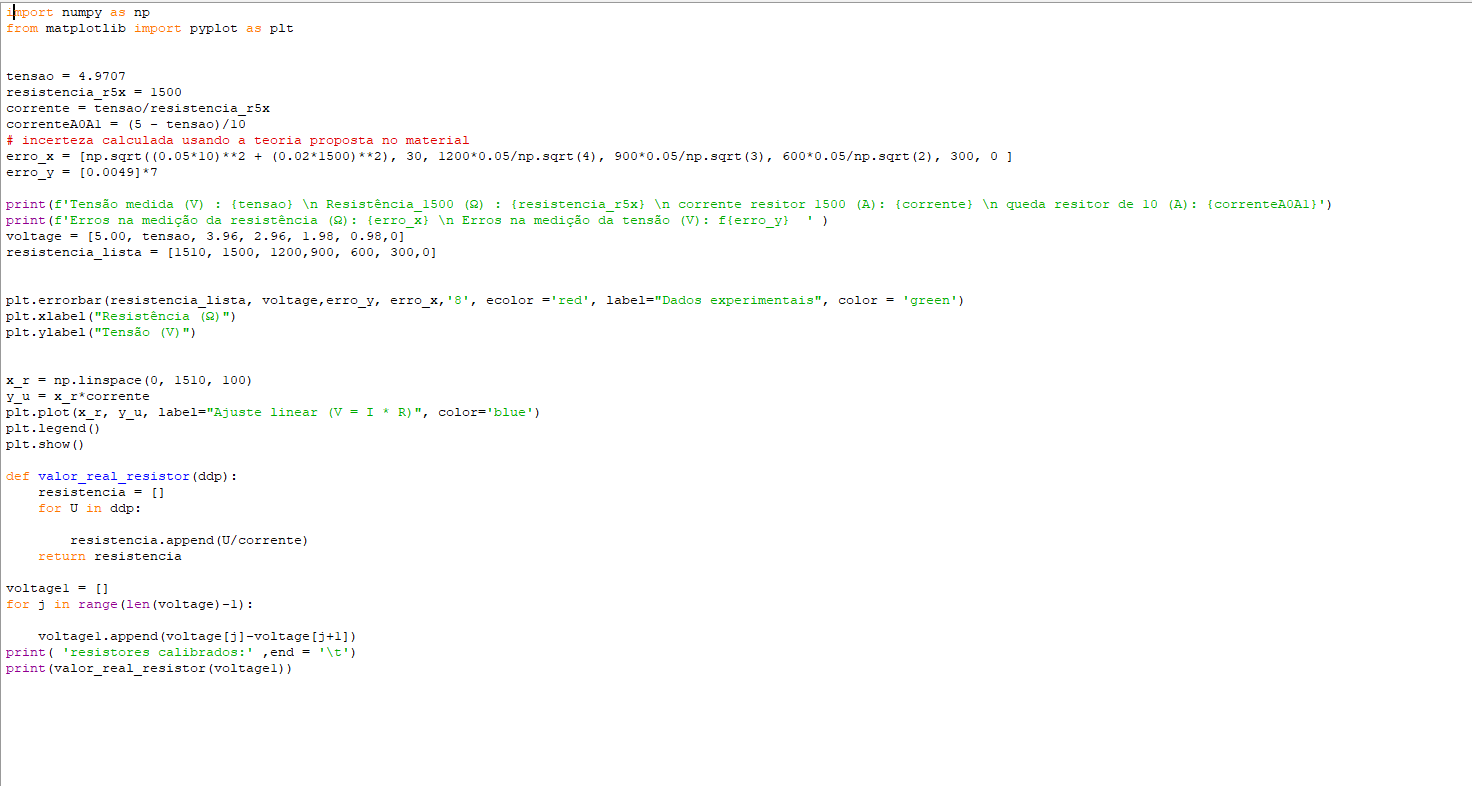
\includegraphics[width=0.8\textwidth]{Código_exp1.png} % Substitua pelo nome do arquivo da imagem
    \caption{Código Python}
    \label{fig:tinkercad}
\end{figure}

\vspace{1em}

\begin{figure}[H]
    \centering
    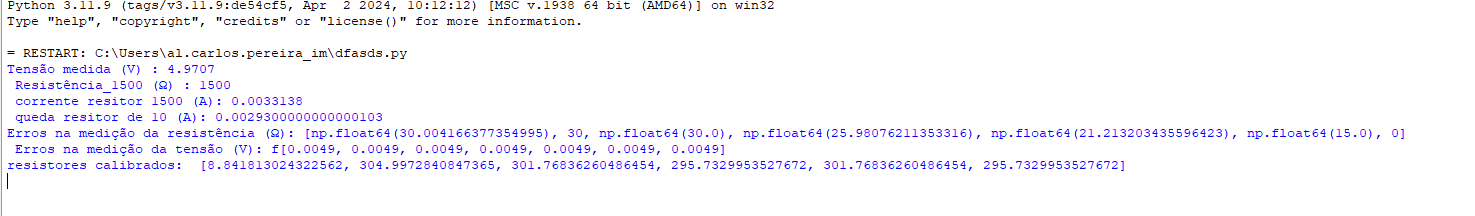
\includegraphics[width=0.8\textwidth]{resultados01.png} % Substitua pelo nome do arquivo da imagem
    \caption{Resultados do Python}
    \label{fig:tinkercad}
\end{figure}

\vspace{1em}

O código começa definindo os valores medidos:
\begin{itemize}
    \item \textbf{Tensão} ($V_{A5}$): Representa a queda de tensão em toda a resistência total do circuito. Aqui, foi medida como 4.9707 V.
    \item \textbf{Resistência Total ($R_{total}$)}: Calculada como a soma de cinco resistores de 300 $\Omega$ (nominais), resultando em 1500 $\Omega$. Com o resistor de 10 $\Omega$ (shunt), o total é $R_{total} = 1510 \, \Omega$.
\end{itemize}

Usando a \textbf{Lei de Ohm} ($I = \frac{V}{R}$), calcula-se:
\begin{itemize}
    \item \textbf{Corrente no circuito principal ($I$)}:
    \[
    I = \frac{4.9707}{1500} \approx 0.0033\pm0.0007~\text{A}.
    \]
    \item \textbf{Corrente medida pelo shunt ($I_{shunt}$)}: 
    Aqui, a corrente é calculada pela queda de tensão no resistor de 10 $\Omega$:
    \[
    I_{shunt} = \frac{5 - 4.9707}{10} \approx 0.00293~\text{A}.
    \]
    Há uma pequena diferença entre $I$ e $I_{shunt}$ devido às limitações de resolução e precisão.
\end{itemize}

\begin{itemize}
    \item CALCULAR AS INCERTEZAS E ADICIONAR EM CADA VALOR (+-)
\end{itemize}

Os dados de tensão medidos ($V$) e as resistências ($R$) associadas são organizados em listas:
\begin{itemize}
    \item Tensão ($V$): $[5.00, 4.9707, 3.96, 2.96, 1.98, 0.98, 0]$.
    \item Resistências ($R$): $[1510, 1500, 1200, 900, 600, 300, 0]$.
\end{itemize}

Esses valores representam os pontos medidos no circuito.

\vspace{1em}

Um gráfico é gerado com:
\begin{itemize}
    \item \textbf{Pontos experimentais}: $V$ em função de $R$, incluindo as barras de erro.
    \item \textbf{Ajuste linear}: Uma linha é ajustada aos dados usando a equação $V = I \cdot R$, onde $I$ é a corrente calculada ($0.003314 \, \text{A}$).
\end{itemize}

Esse gráfico é importante para verificar a proporcionalidade entre $V$ e $R$, confirmando a Lei de Ohm.


\vspace{1em}

\begin{figure}[H]
    \centering
    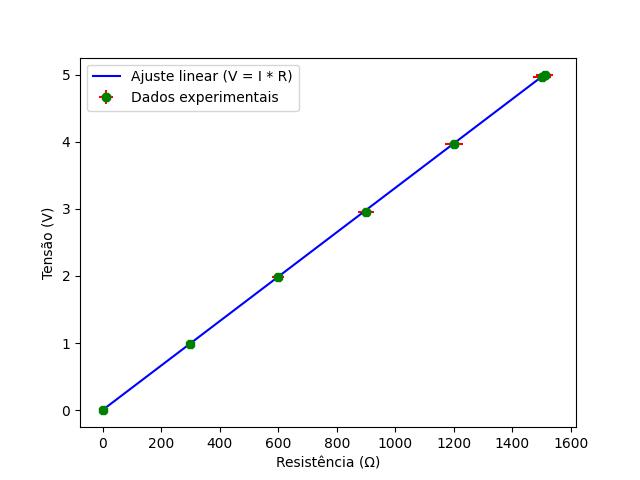
\includegraphics[width=0.8\textwidth]{GráficoUxR.png} % Substitua pelo nome do arquivo da imagem
    \caption{Gráfico V x R}
    \label{fig:tinkercad}
\end{figure}

O código utiliza as quedas de tensão entre os pontos ($\Delta V = V_{n} - V_{n+1}$) para calcular os valores reais dos resistores. A fórmula aplicada é novamente a Lei de Ohm:
\[
R = \frac{\Delta V}{I}.
\]

\begin{itemize}

    \item \textbf{Resistor 1 (R1):}
    \[
    \Delta V = V_1 - V_2 = 4.9707 - 3.96 = 1.0107 \, \text{V}
    \]
    \[
    R_2 = \frac{\Delta V}{I} = \frac{1.0107}{0.0033138} \approx 305.00 \, \Omega
    \]

    \item \textbf{Resistor 2 (R2):}
    \[
    \Delta V = V_2 - V_3 = 3.96 - 2.96 = 1.00 \, \text{V}
    \]
    \[
    R_3 = \frac{\Delta V}{I} = \frac{1.00}{0.0033138} \approx 301.77 \, \Omega
    \]

    \item \textbf{Resistor 3 (R3):}
    \[
    \Delta V = V_3 - V_4 = 2.96 - 1.98 = 0.98 \, \text{V}
    \]
    \[
    R_4 = \frac{\Delta V}{I} = \frac{0.98}{0.0033138} \approx 295.73 \, \Omega
    \]

    \item \textbf{Resistor 4 (R4):}
    \[
    \Delta V = V_4 - V_5 = 1.98 - 0.98 = 1.00 \, \text{V}
    \]
    \[
    R_5 = \frac{\Delta V}{I} = \frac{1.00}{0.0033138} \approx 301.77 \, \Omega
    \]

    \item \textbf{Resistor 5 (R5):}
    \[
    \Delta V = V_5 - V_6 = 0.98 - 0.00 = 0.98 \, \text{V}
    \]
    \[
    R_6 = \frac{\Delta V}{I} = \frac{0.98}{0.0033138} \approx 295.73 \, \Omega
    \]
\end{itemize}

Esses valores são usados para ajustar os resistores nominalmente de 300 $\Omega$ e garantir maior precisão no circuito.


\vspace{1em}
\begin{table}[ht]
    \centering
    \begin{tabular}{|c|c|}
        \hline
        Resistor & Resistência ($\Omega$) \\
        \hline
        1 & 305.00 \\
        2 & 301.77 \\
        3 & 295.73 \\
        4 & 301.77 \\
        5 & 295.73 \\
        \hline
    \end{tabular}
    \caption{Resistências Calibradas}
    \label{tab:tensoes}
\end{table}


\subsection{Conclusão}
\leavevmode

TIVEMOS RESULTADOS ESPERADOS? A LEI DE OHM FOI VERIFICADA? EXPLICAÇÃO DOS NOSSOS DADOS?

\section{Calibração de 3 shunts de 10 $\Omega$ e R_l's}

\subsection{Introdução}
\leavevmode

A calibração de resistores é uma etapa fundamental para assegurar precisão e confiabilidade em medições elétricas. Este experimento tem como objetivo calibrar três resistores shunt de aproximadamente 10 Ω, utilizando métodos de medição de tensão e cálculo de corrente para determinar com maior exatidão os valores reais desses componentes.

A calibração é realizada por meio de um circuito que permite avaliar a relação entre a corrente elétrica e a queda de tensão nos resistores. A partir dessas medições, é possível calcular com precisão o valor de resistência dos shunts, corrigindo eventuais discrepâncias em relação ao valor nominal indicado pelo fabricante. Essa abordagem é essencial para garantir a eficiência de sistemas que dependem da leitura precisa de correntes e tensões.

Os resultados obtidos serão registrados para assegurar que os resistores calibrados possam ser utilizados em futuras aplicações com maior grau de confiabilidade. Este experimento reforça a importância da calibração como prática indispensável no desenvolvimento e manutenção de sistemas eletrônicos.

\subsection{Montagem}
\leavevmode

Assim como no experimento anterior, antes de toda montagem do experimento físico, foi realizada uma simulação no ambiente virtual do TinkerCad do nosso circuito, EXPLICAÇÃO DA MONTAGEM. Ademais, criamos um código (.ino) para conseguirmos realizar o experimento 2.

\vspace{1em}

\begin{figure}[H]
    \centering
    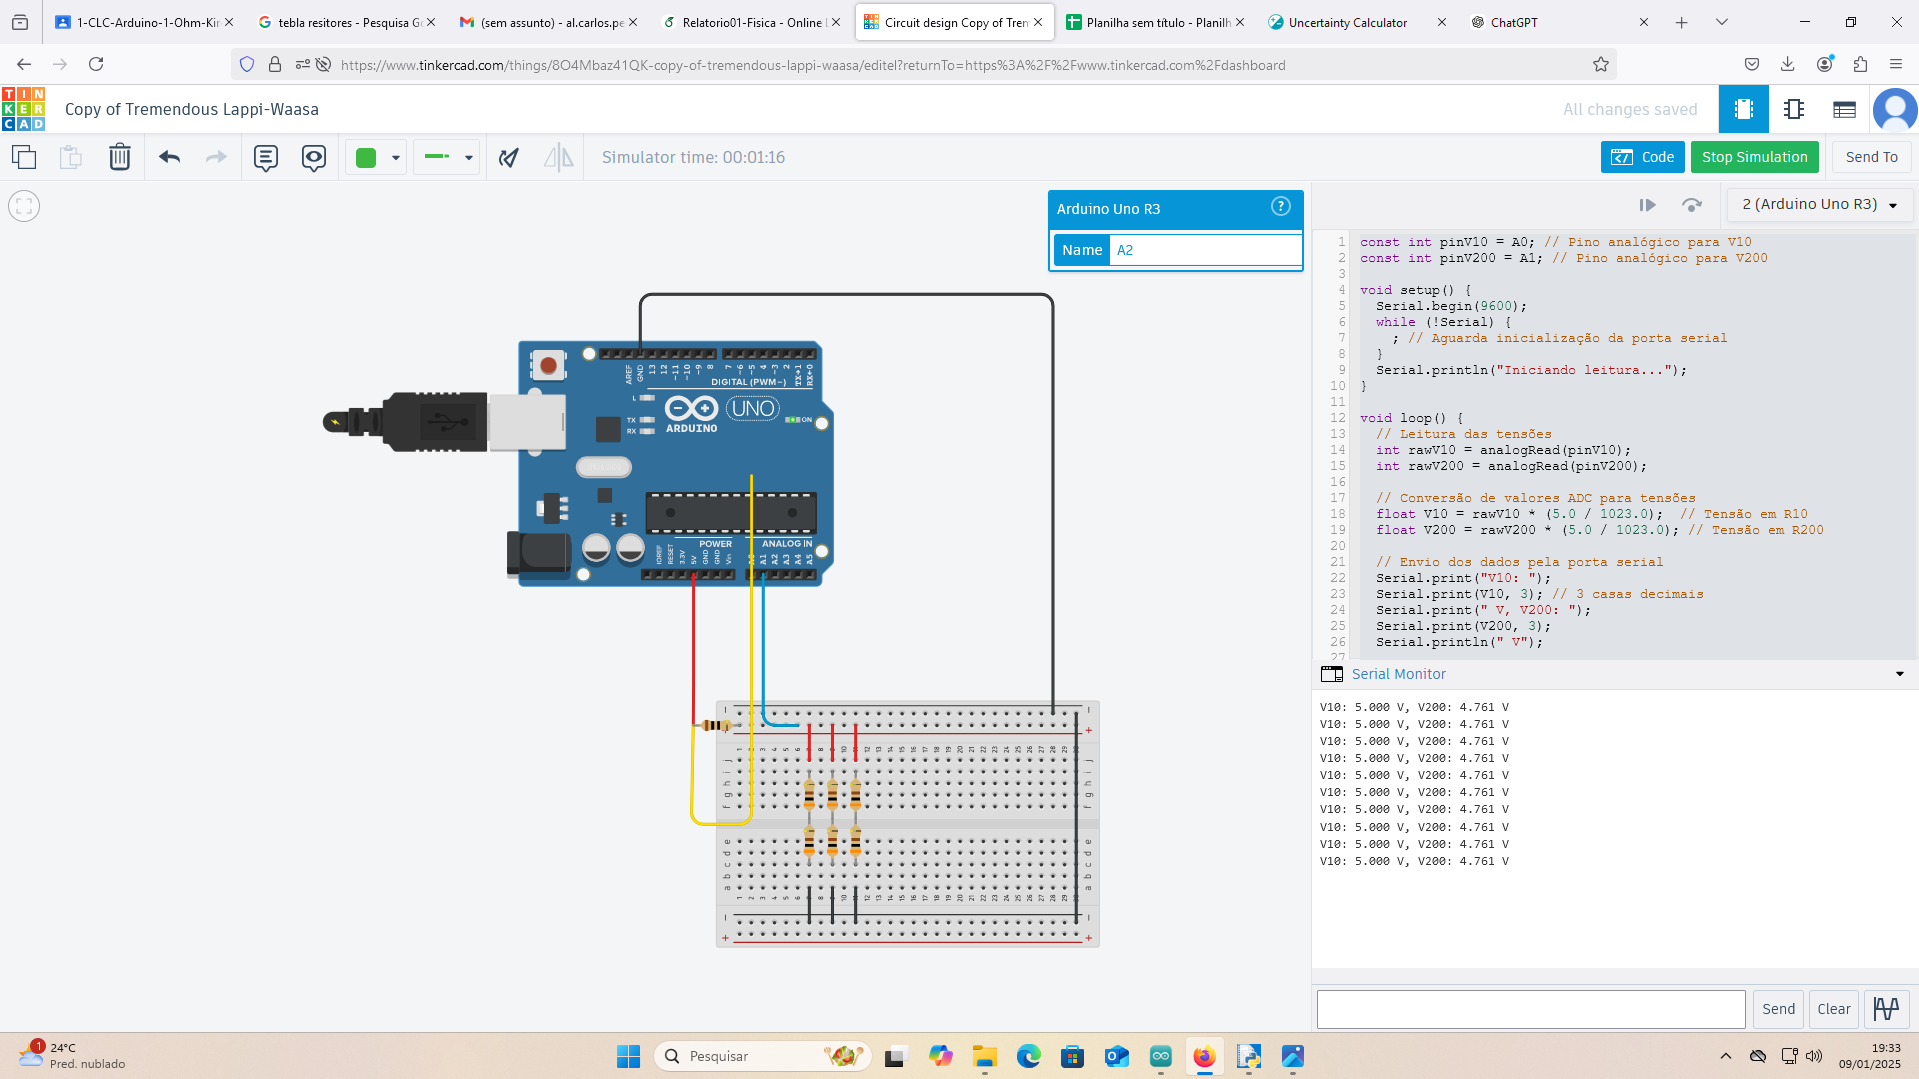
\includegraphics[width=0.8\textwidth]{Captura de tela 2025-01-09 193315.png} % Substitua pelo nome do arquivo da imagem
    \caption{Simulação do circuito no TinkerCad.}
    \label{fig:tinkercad}
\end{figure}

\vspace{1em}

Logo após essa simulação no TinkerCad, reproduzimos o circuito no Arduino Uno para comparação dos dados obtidos.

\vspace{1em}

\begin{figure}[H]
    \centering
    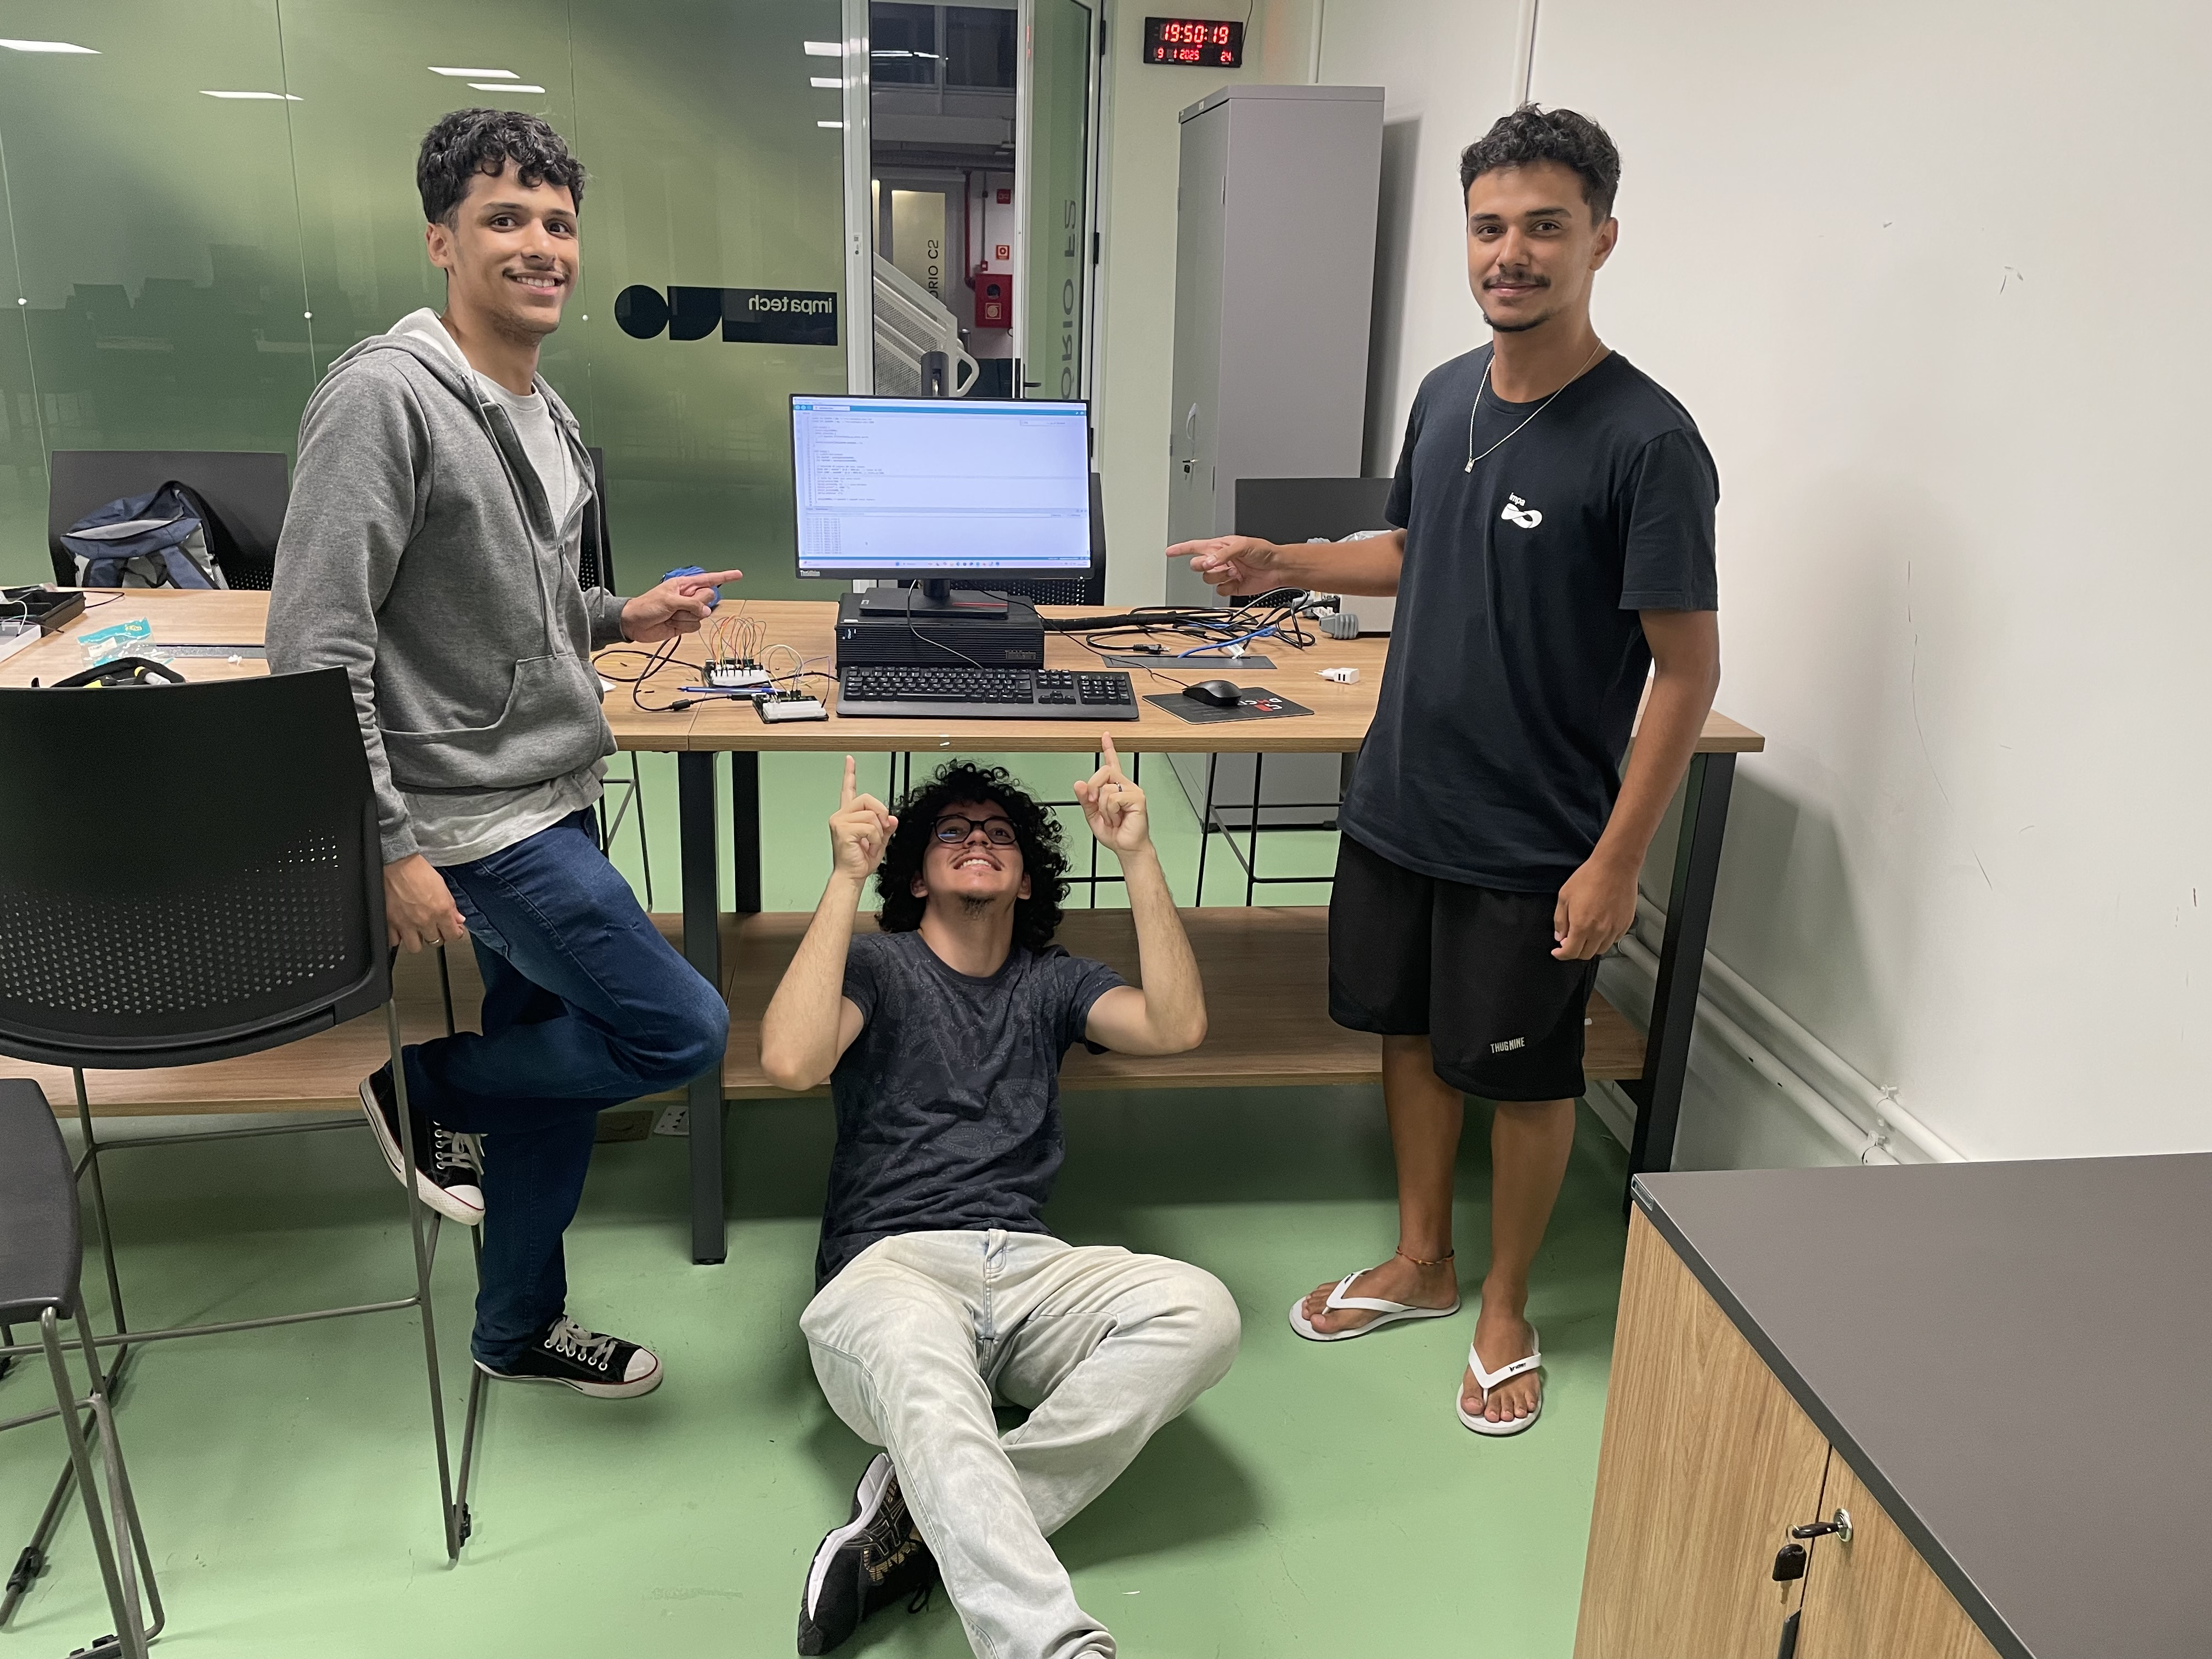
\includegraphics[width=0.8\textwidth]{IMG_1148.jpg} % Substitua pelo nome do arquivo da imagem
    \caption{Montagem do experimento pelos integrantes do grupo.}
    \label{fig:arduino}
\end{figure}

\vspace{1em}
\begin{figure}[H]
    \centering
    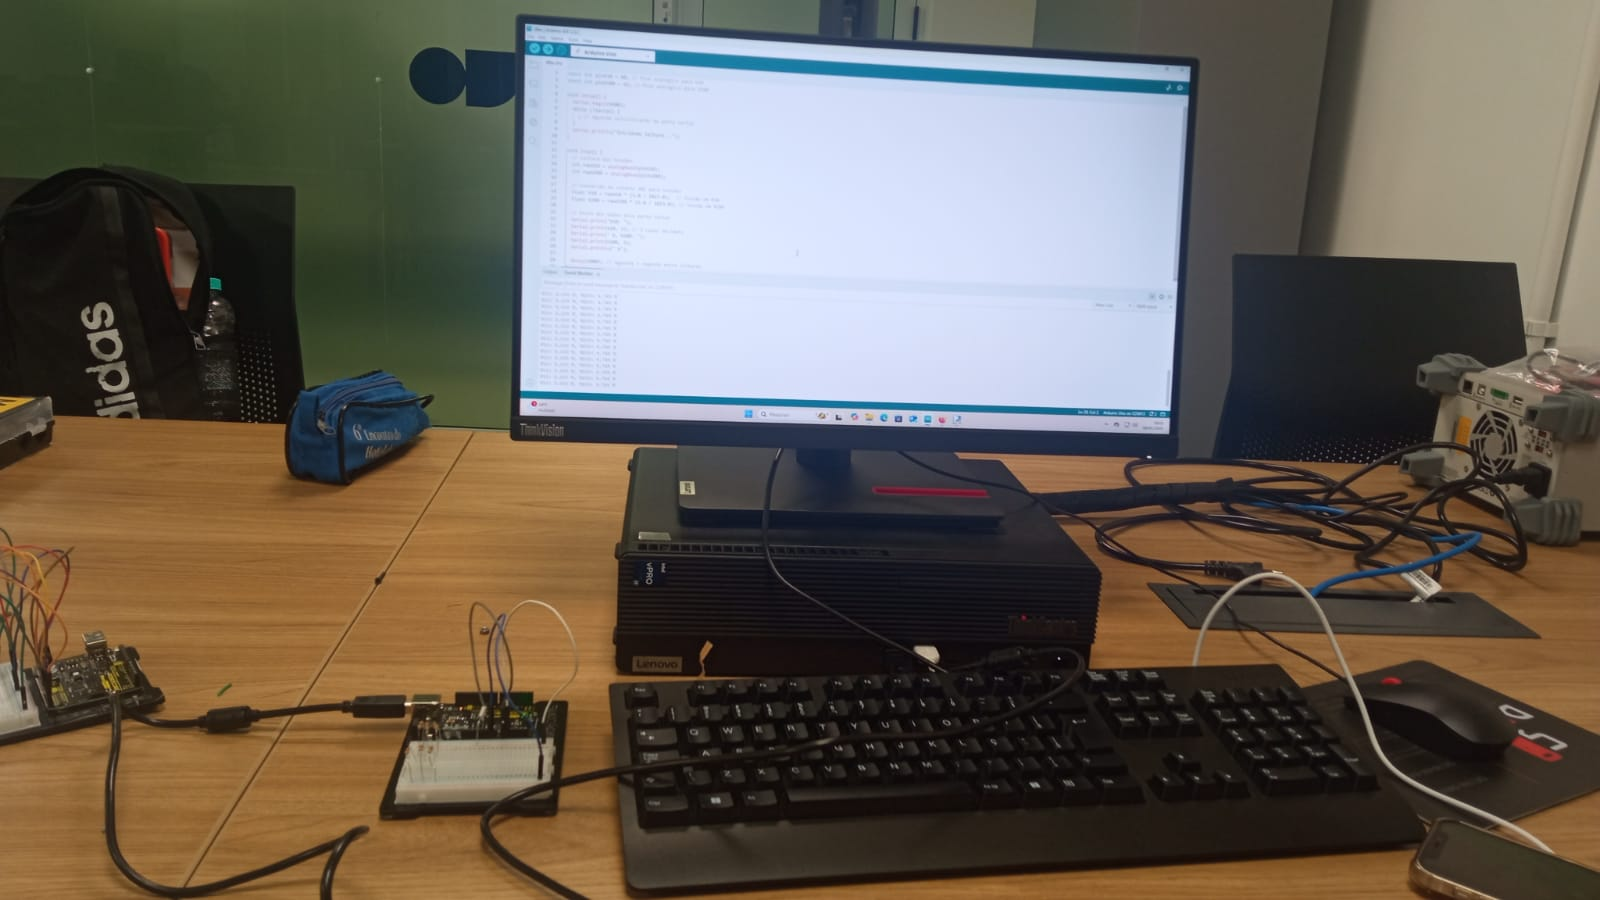
\includegraphics[width=0.8\textwidth]{FOTO 1.jpg} % Substitua pelo nome do arquivo da imagem
    \caption{Circuito montado no Arduino Uno.}
    \label{fig:arduino}
\end{figure}

\vspace{1em}

\begin{figure}[H]
    \centering
    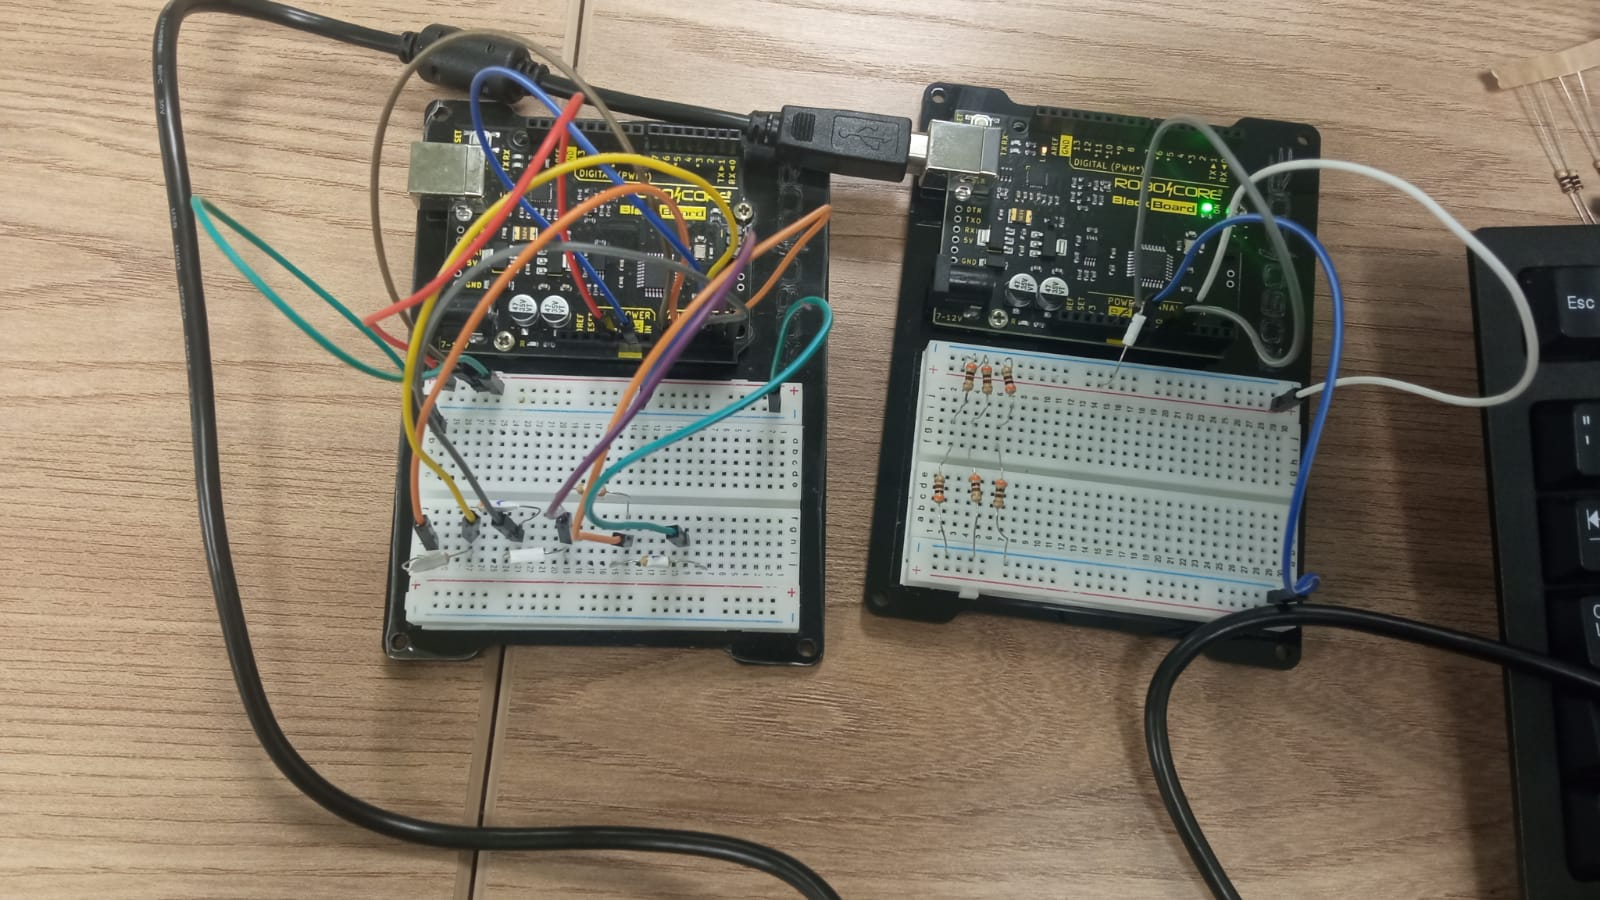
\includegraphics[width=0.8\textwidth]{FOTO 2.jpg} % Substitua pelo nome do arquivo da imagem
    \caption{Circuito montado no Arduino Uno.}
    \label{fig:arduino}
\end{figure}

\vspace{1em}

\subsection{Resultados}
\subsubsection{Dados}
\leavevmode

Depois de toda a simulação e a realização do experimento no Arduino Uno, obtivemos os seguintes valores das tensões de V10 e V200:

\vspace{1em}

\begin{figure}[H]
    \centering
    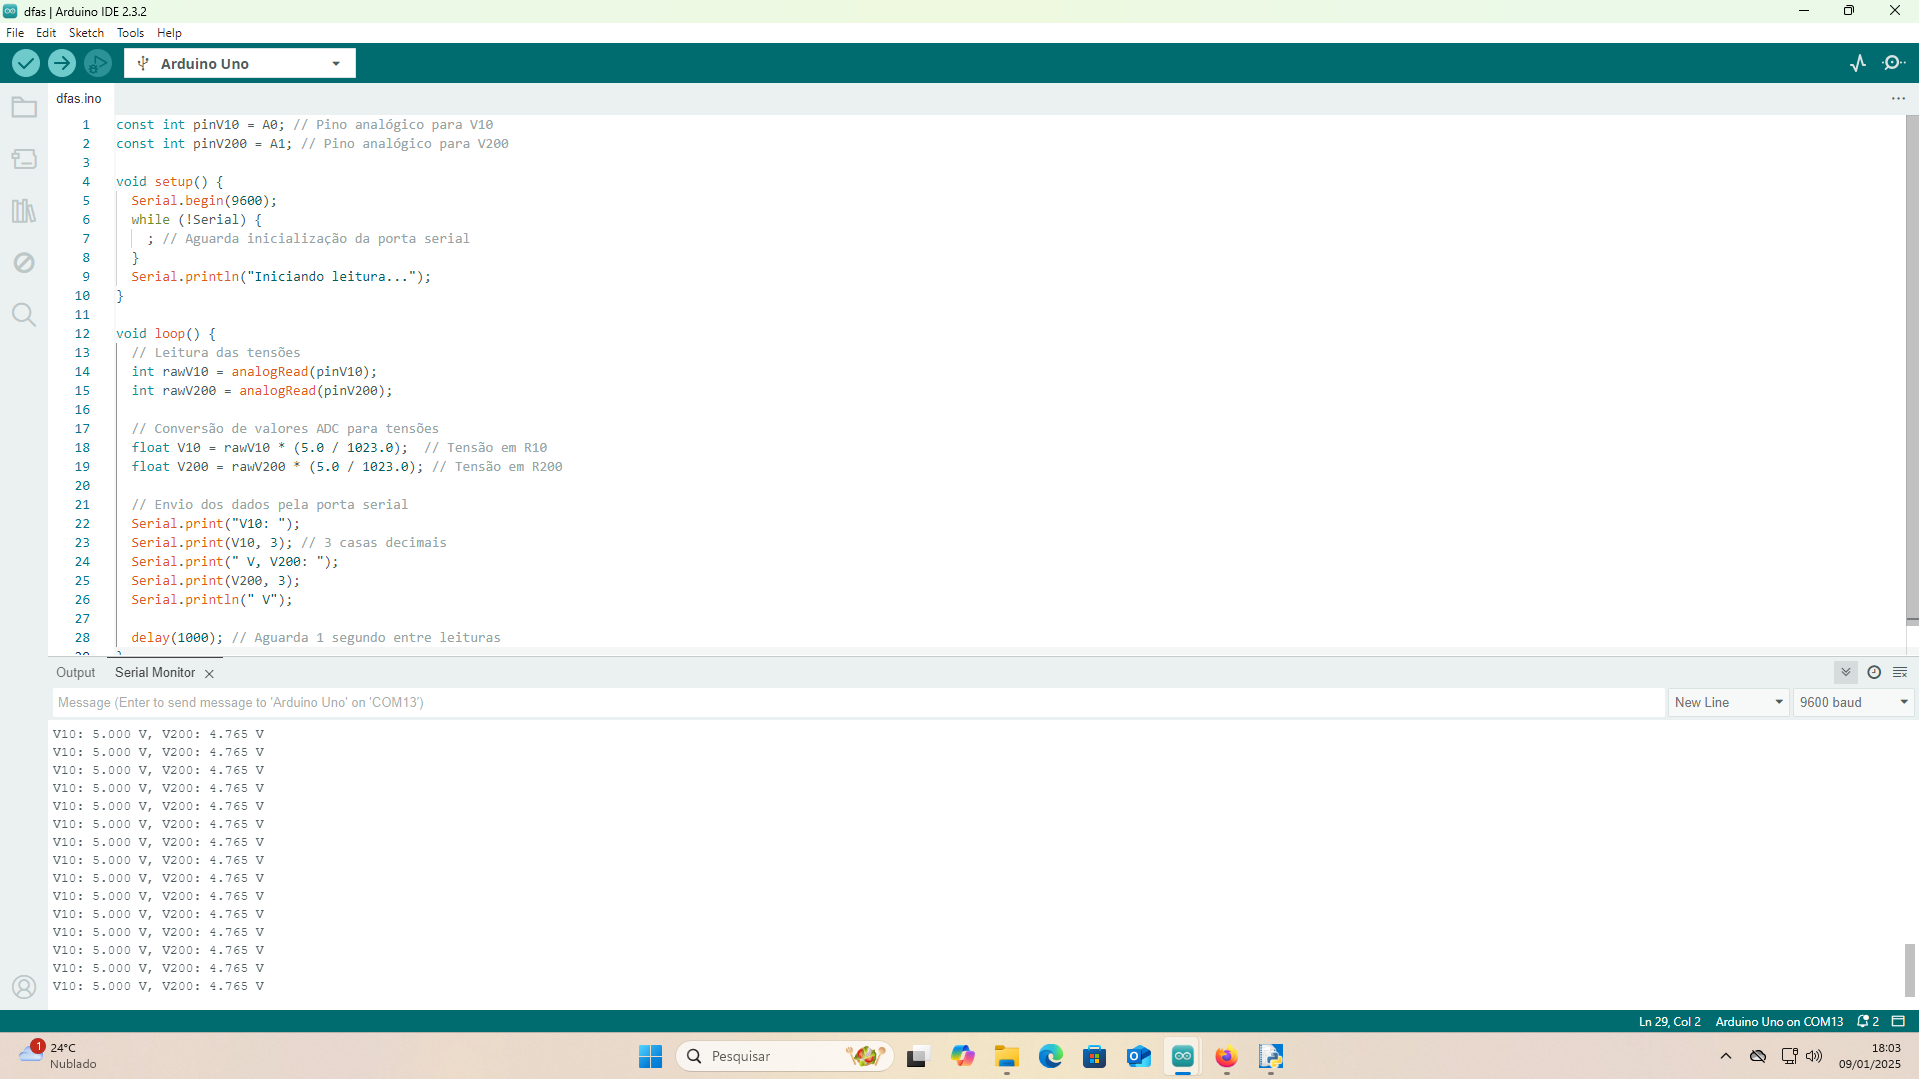
\includegraphics[width=0.8\textwidth]{A.png} % Substitua pelo nome do arquivo da imagem
    \caption{Tensões Obtidas - Resistor A}
    \label{fig:arduino}
\end{figure}

\vspace{1em}

\begin{figure}[H]
    \centering
    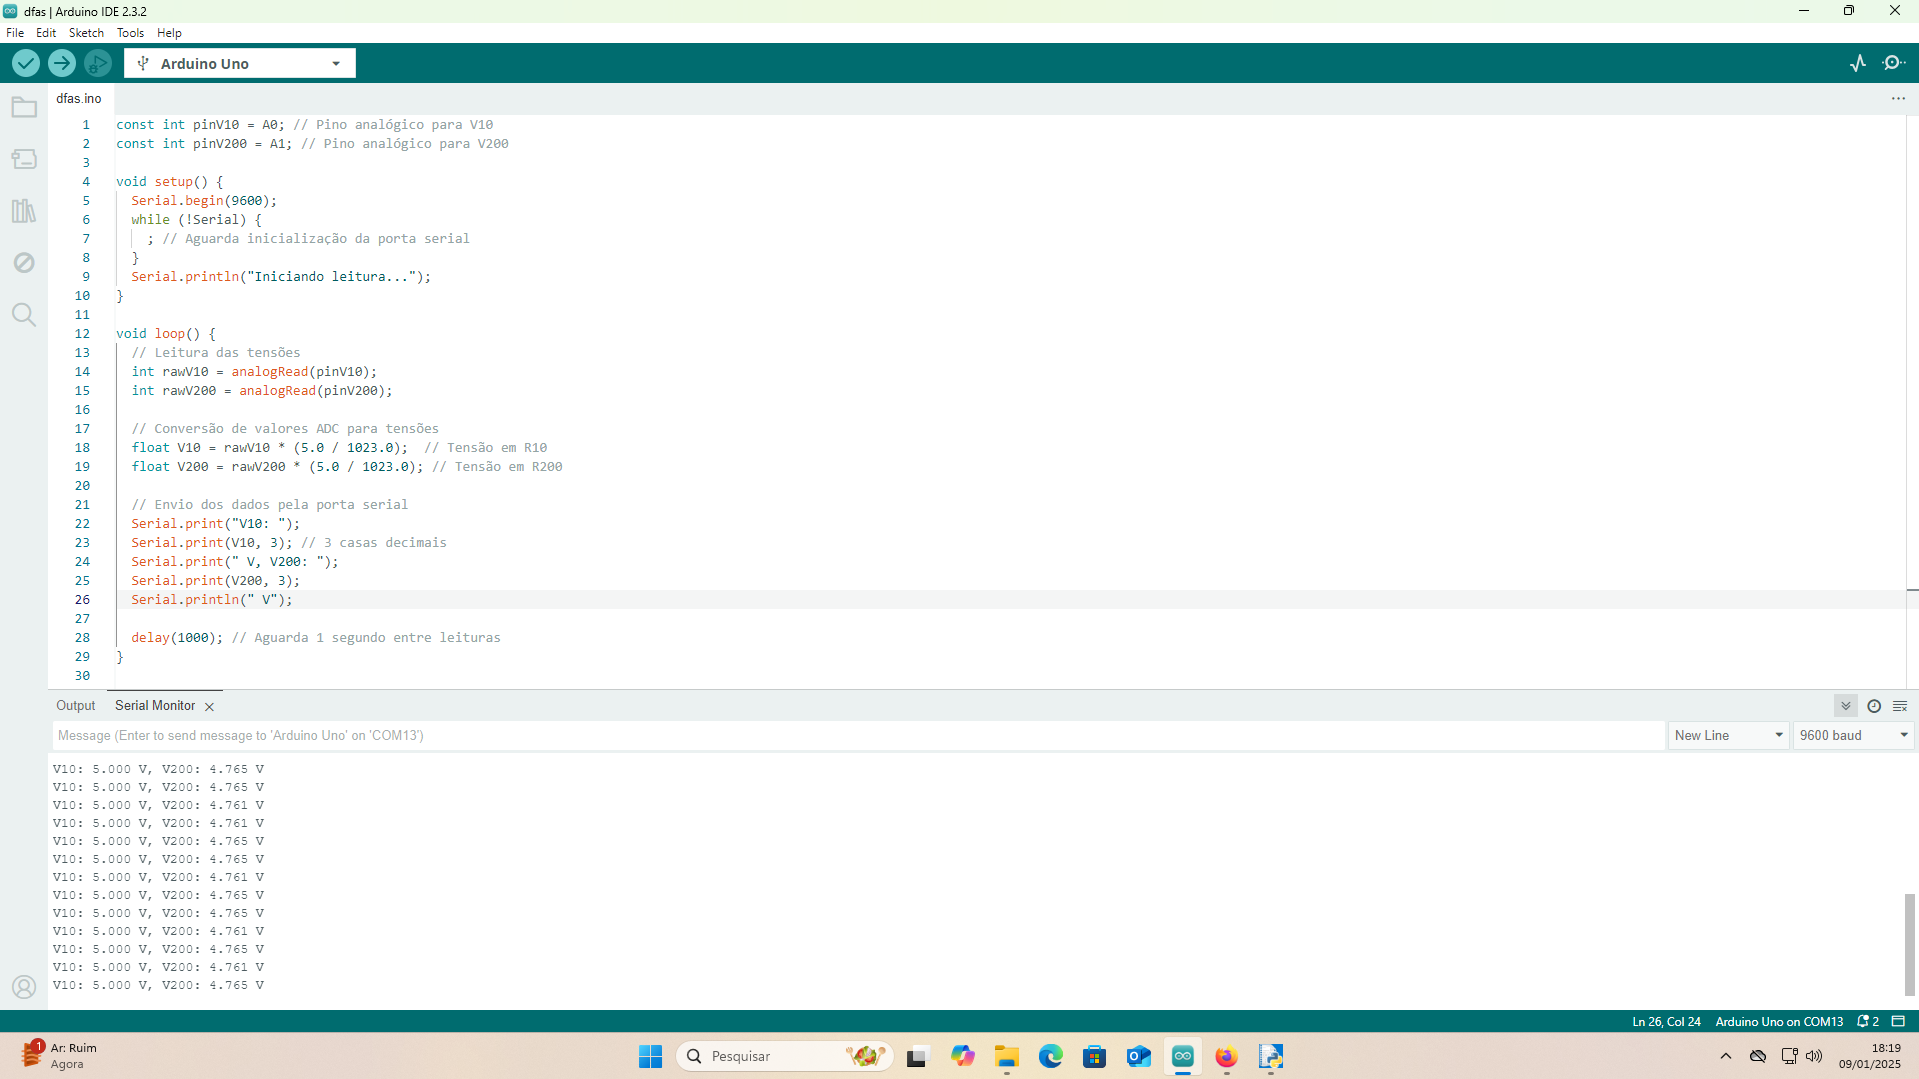
\includegraphics[width=0.8\textwidth]{B.png} % Substitua pelo nome do arquivo da imagem
    \caption{Tensões Obtidas - Resistor B}
    \label{fig:arduino}
\end{figure}

\vspace{1em}

\begin{figure}[H]
    \centering
    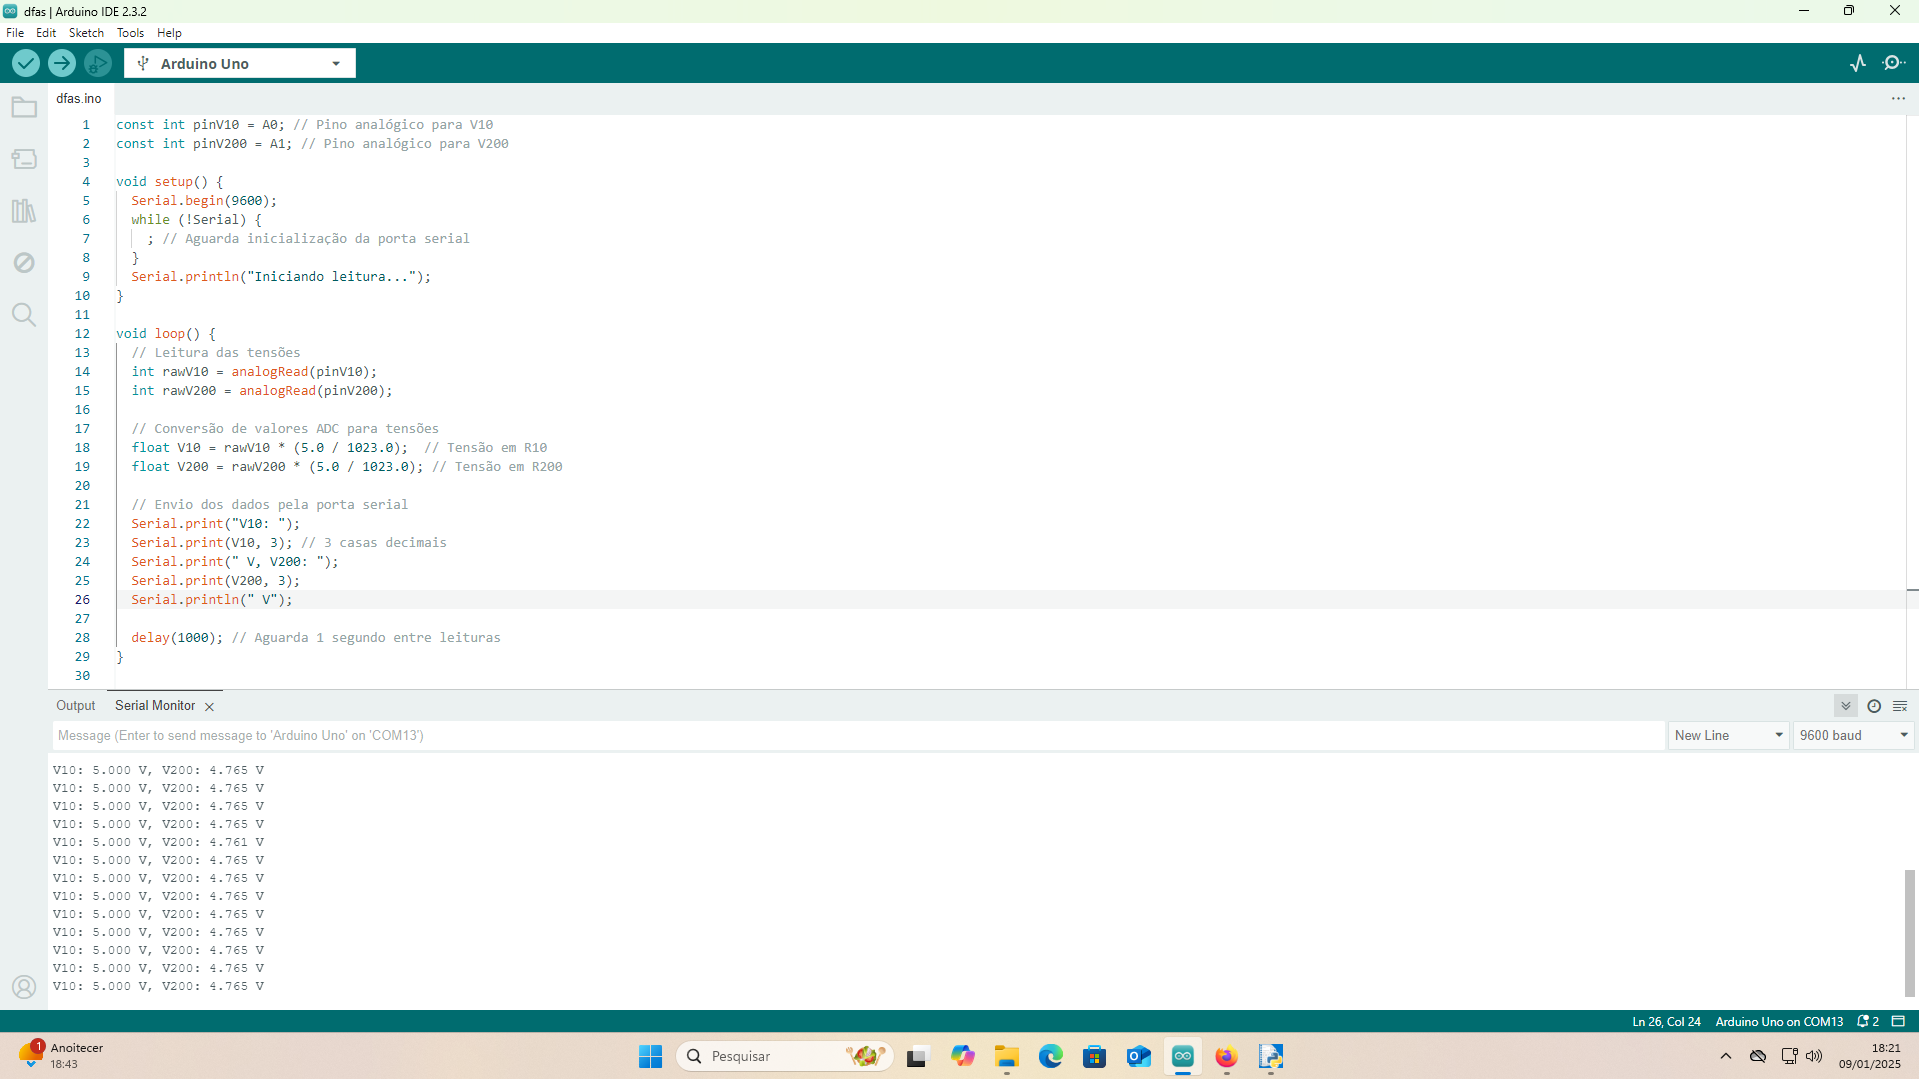
\includegraphics[width=0.8\textwidth]{C.png} % Substitua pelo nome do arquivo da imagem
    \caption{Tensões Obtidas - Resistor C}
    \label{fig:arduino}
\end{figure}

\vspace{1em}


\begin{table}[ht]
\centering
\begin{tabular}{|c|c|c|}
\hline
\textbf{Resistor} & \textbf{Tensão - V10 (V)} & \textbf{Tensão - V200 (V)} \\
\hline
A & 5.00 & 4.76 \\
\hline
B & 5.00 & 4.76 \\
\hline
C & 5.00 & 4.76 \\
\hline
\end{tabular}
\caption{Tensões obtidas de cada resistor}
\end{table}

\vspace{1em}

\subsubsection{Calibração}
\leavevmode

ANALISAR TODOS DADOS, SE TIVER CODIGO POR E EXPLICAR, COLOCAR FORMULAS E CONTAS E OS NOSSOS RESULTADOS

\subsection{Conclusão}
\leavevmode

MERMA COISA DO OUTRO

\section{Divisão de corrente em circuito paralelo e soma das correntes em um nó}

\subsection{Introdução}
\leavevmode

Este experimento tem como objetivo analisar a divisão de corrente em circuitos paralelos e verificar a aplicação da Lei de Kirchhoff dos Nós. Através da medição de tensões e cálculo de correntes em diferentes partes do circuito, será possível compreender como a corrente total se distribui entre os braços paralelos e como essa soma se relaciona com a corrente total que percorre o circuito.

Além disso, serão avaliadas as resistências equivalentes e as discrepâncias entre os valores teóricos e medidos das correntes, reforçando a importância da precisão em medições e cálculos elétricos. Por fim, será realizada uma verificação prática da validade da Lei de Kirchhoff, comparando a soma das correntes nos braços paralelos com a corrente total do circuito. 

Esse experimento contribui para a compreensão de princípios fundamentais da análise de circuitos, combinando teoria e prática para validar conceitos como a divisão de corrente e a conservação de carga em nós.

\subsection{Montagem}
\leavevmode

Assim como nos demais experimentos, antes de toda montagem do experimento físico, foi realizada uma simulação no ambiente virtual do TinkerCad do nosso circuito, EXPLICAÇÃO DA MONTAGEM. Ademais, fizemos uso do código (.ino) do Voltimetro disponibilizado pelo professor para extrair os dados do circuito.

\vspace{1em}

\begin{figure}[H]
    \centering
    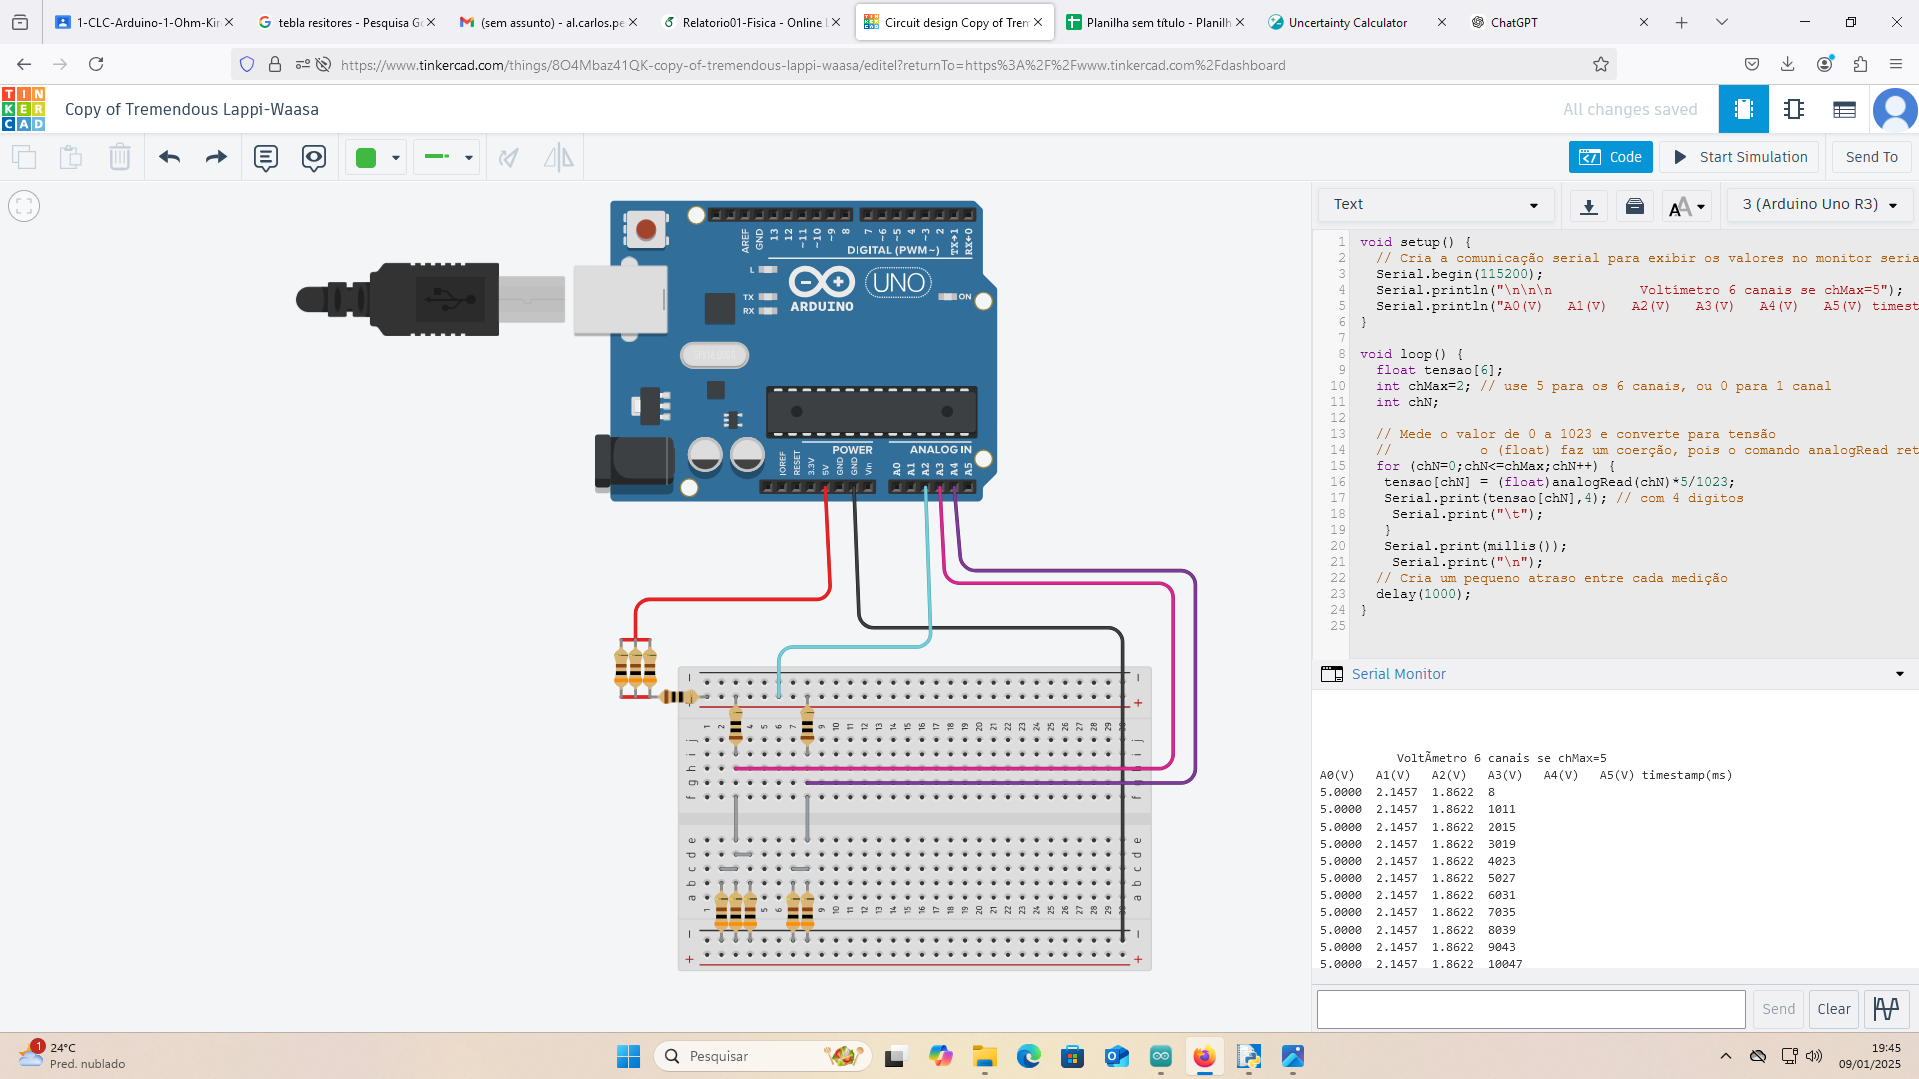
\includegraphics[width=0.8\textwidth]{Captura de tela 2025-01-09 194527.png} % Substitua pelo nome do arquivo da imagem
    \caption{Simulação do circuito no TinkerCad.}
    \label{fig:tinkercad}
\end{figure}

\vspace{1em}

Logo após essa simulação no TinkerCad, reproduzimos o circuito no Arduino Uno para comparação dos dados obtidos.

\vspace{1em}

\begin{figure}[H]
    \centering
    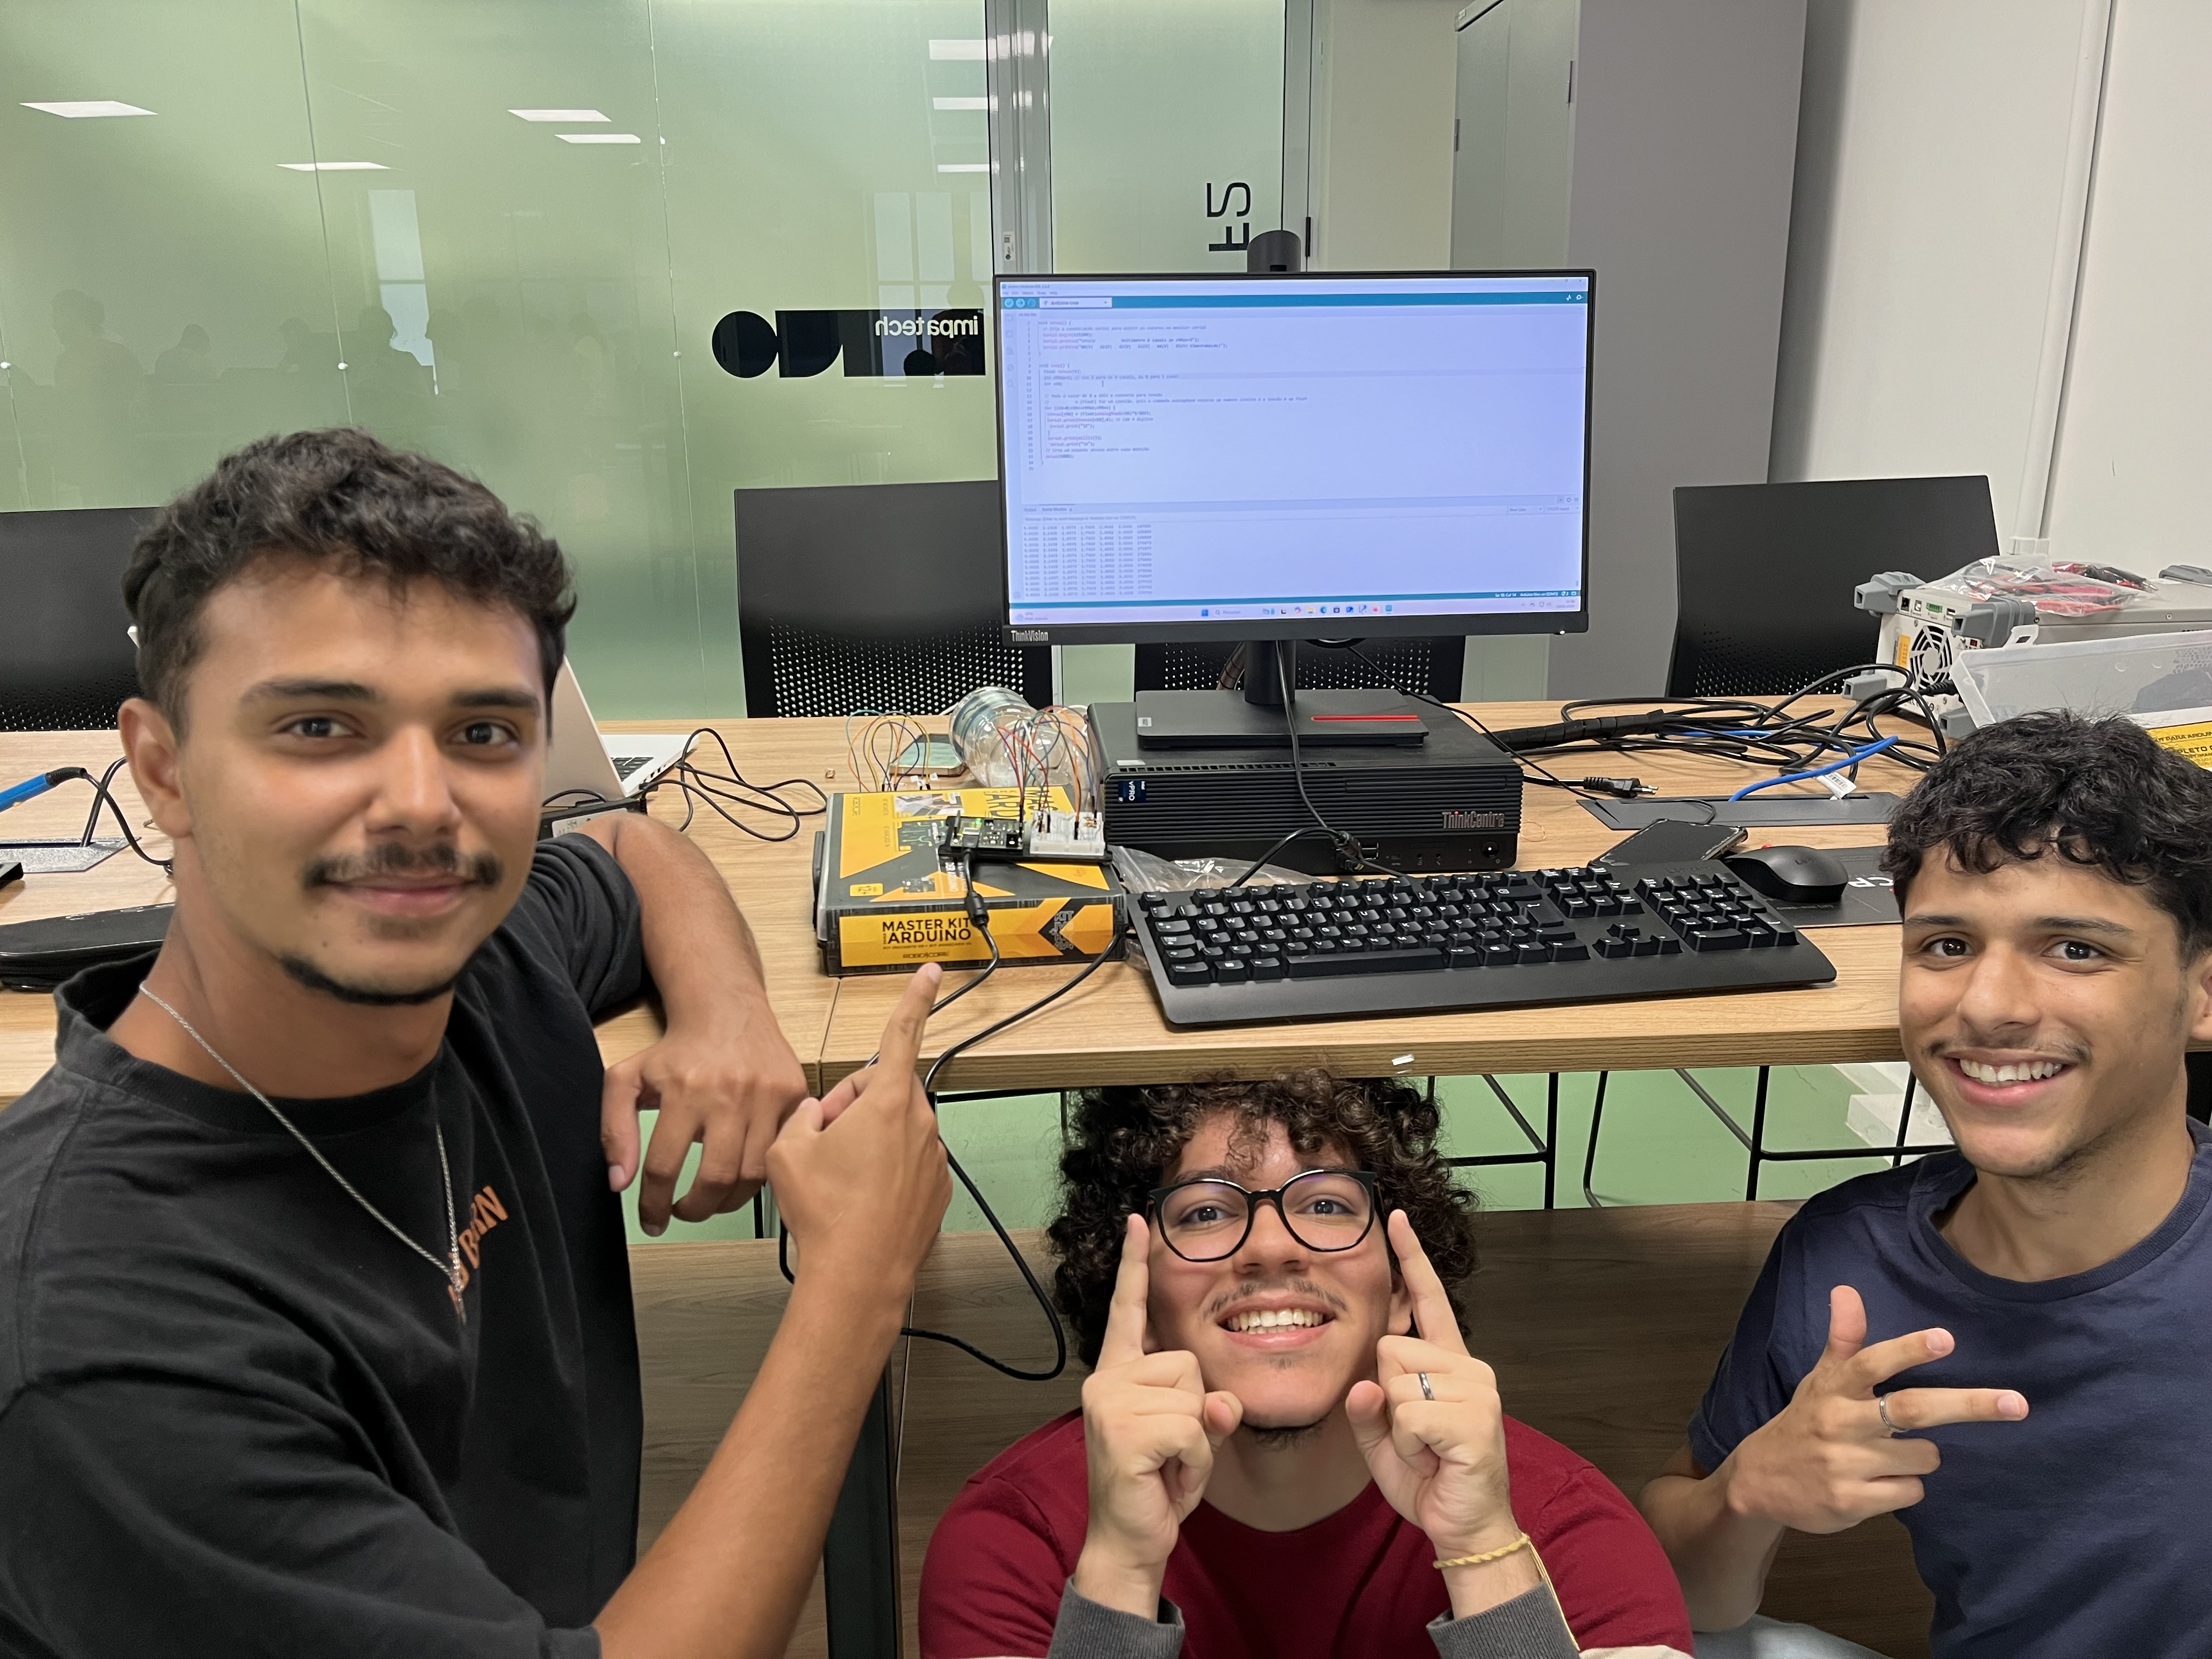
\includegraphics[width=0.8\textwidth]{IMG_3624.jpg} % Substitua pelo nome do arquivo da imagem
    \caption{Montagem do experimento pelos integrantes do grupo.}
    \label{fig:arduino}
\end{figure}

\vspace{1em}
\begin{figure}[H]
    \centering
    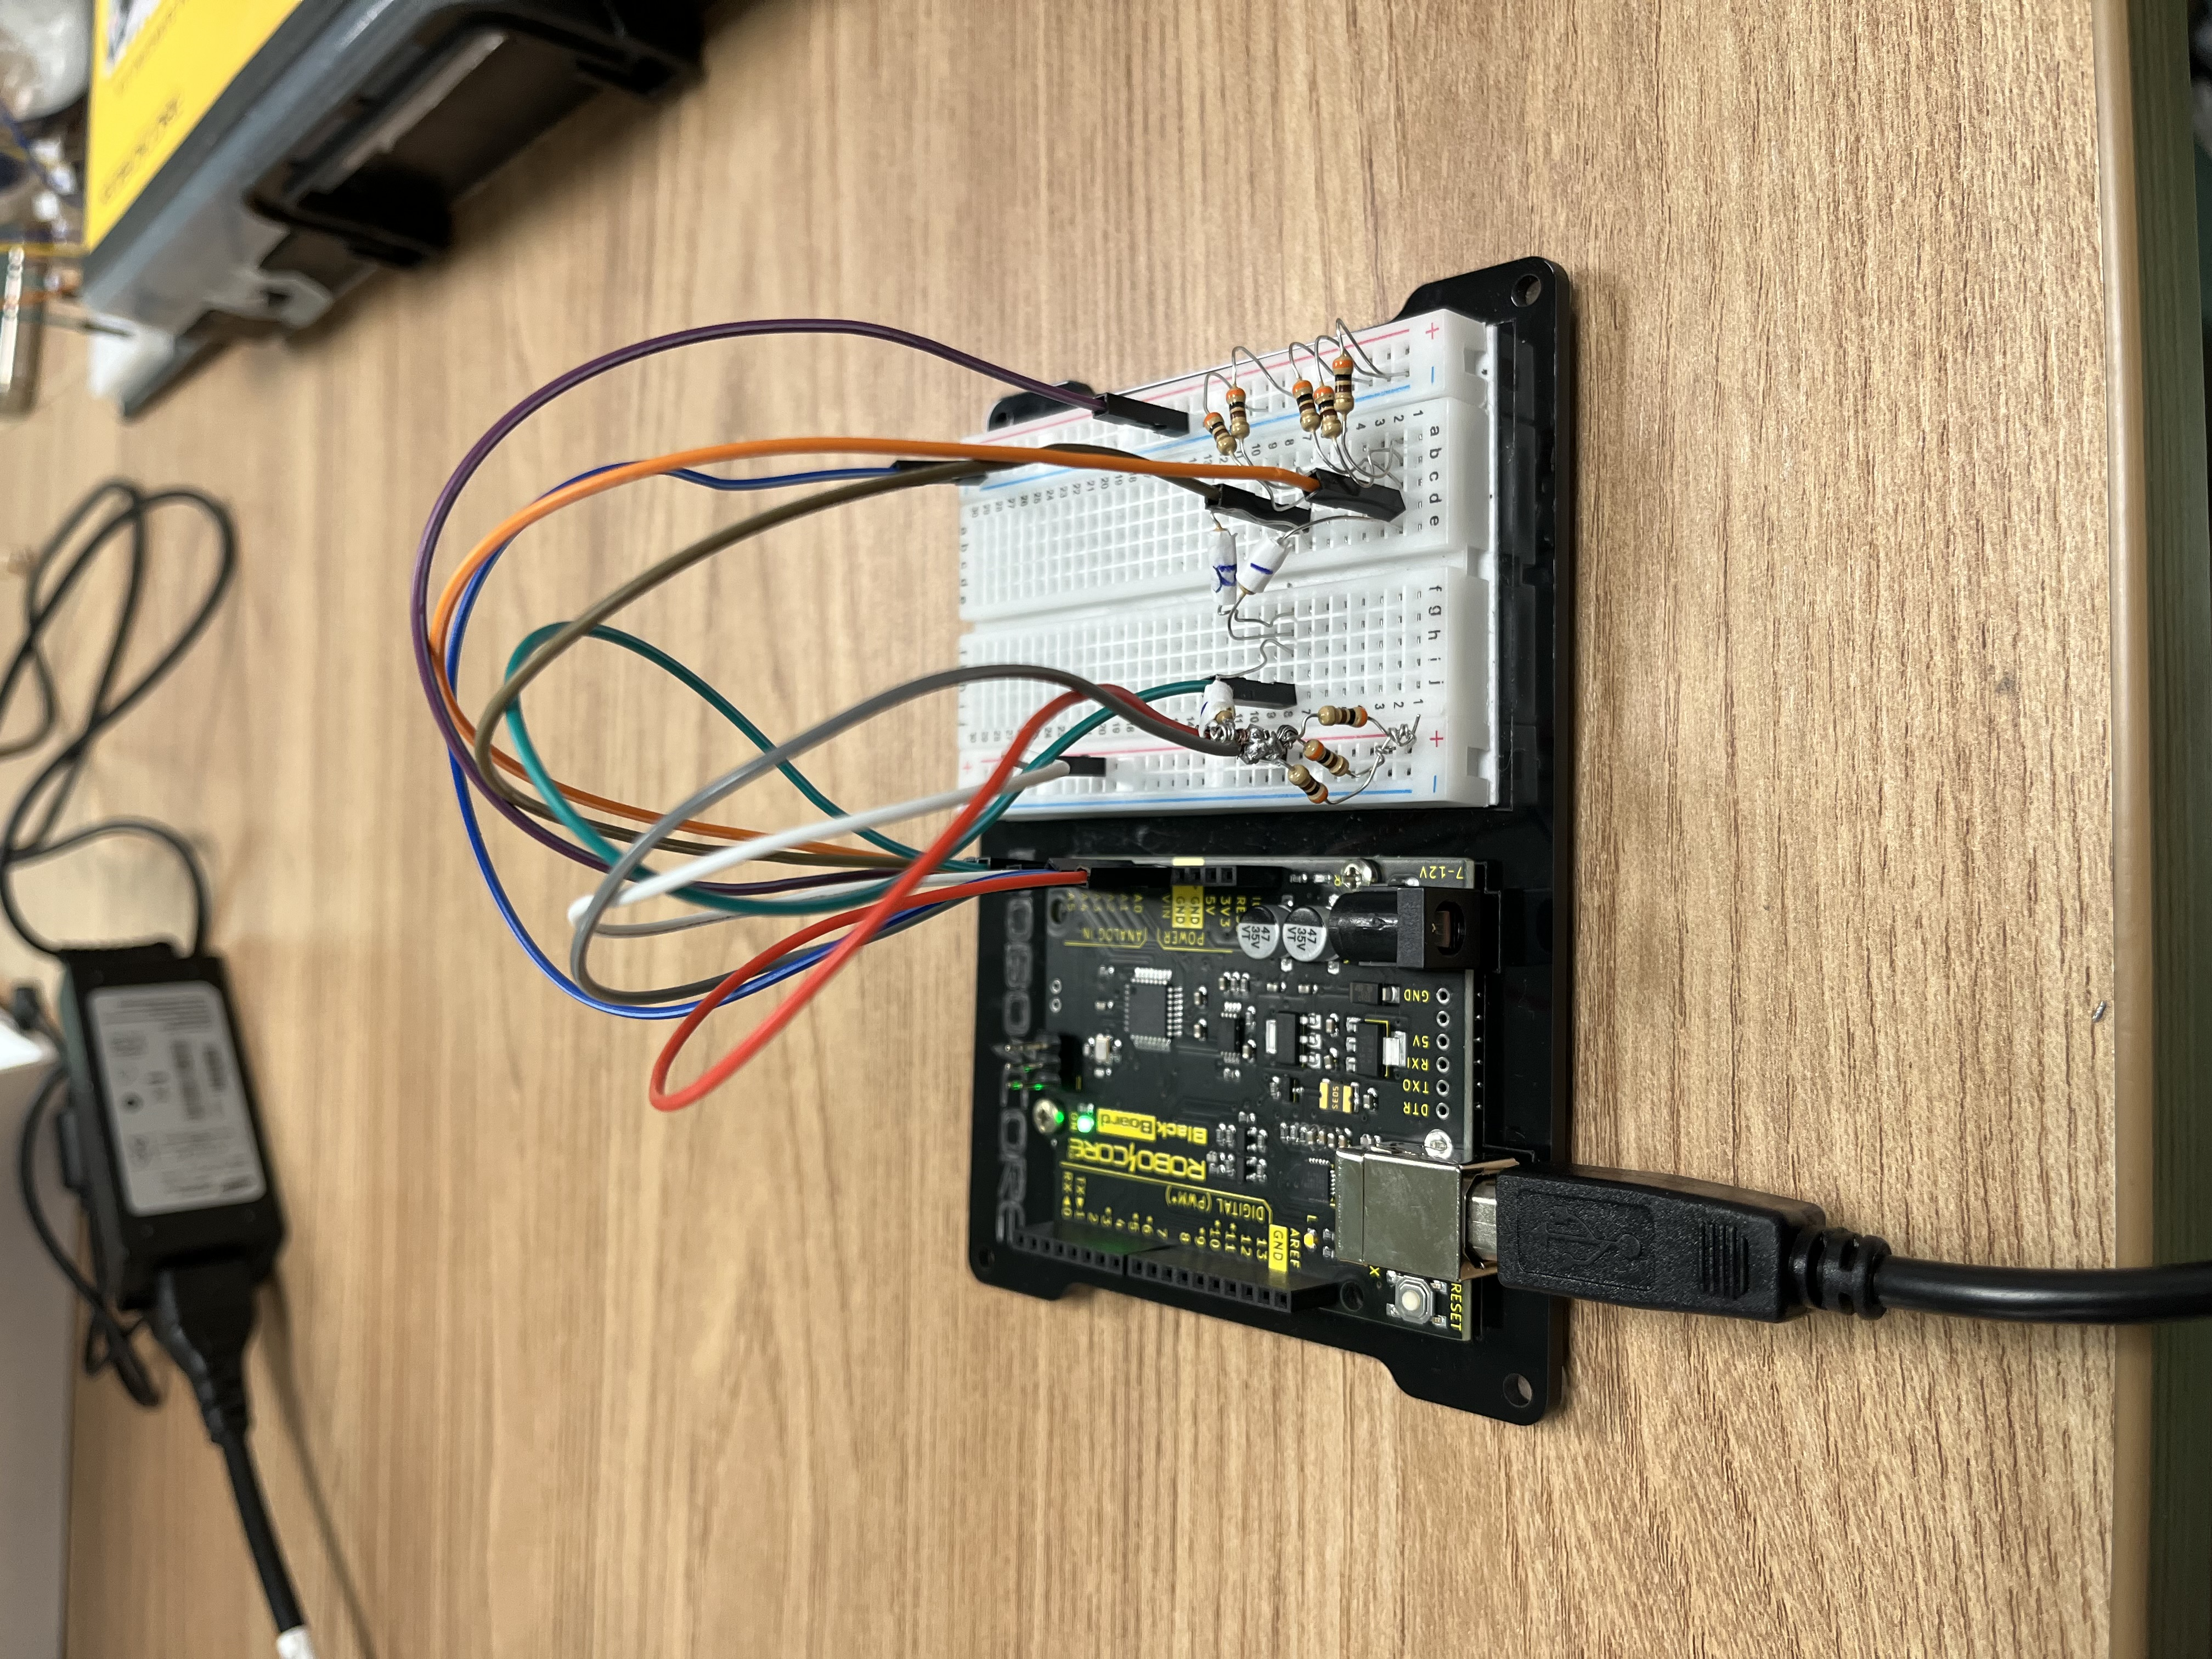
\includegraphics[width=0.8\textwidth]{IMG_3620.jpg} % Substitua pelo nome do arquivo da imagem
    \caption{Circuito montado no Arduino Uno.}
    \label{fig:arduino}
\end{figure}

\vspace{1em}

\begin{figure}[H]
    \centering
    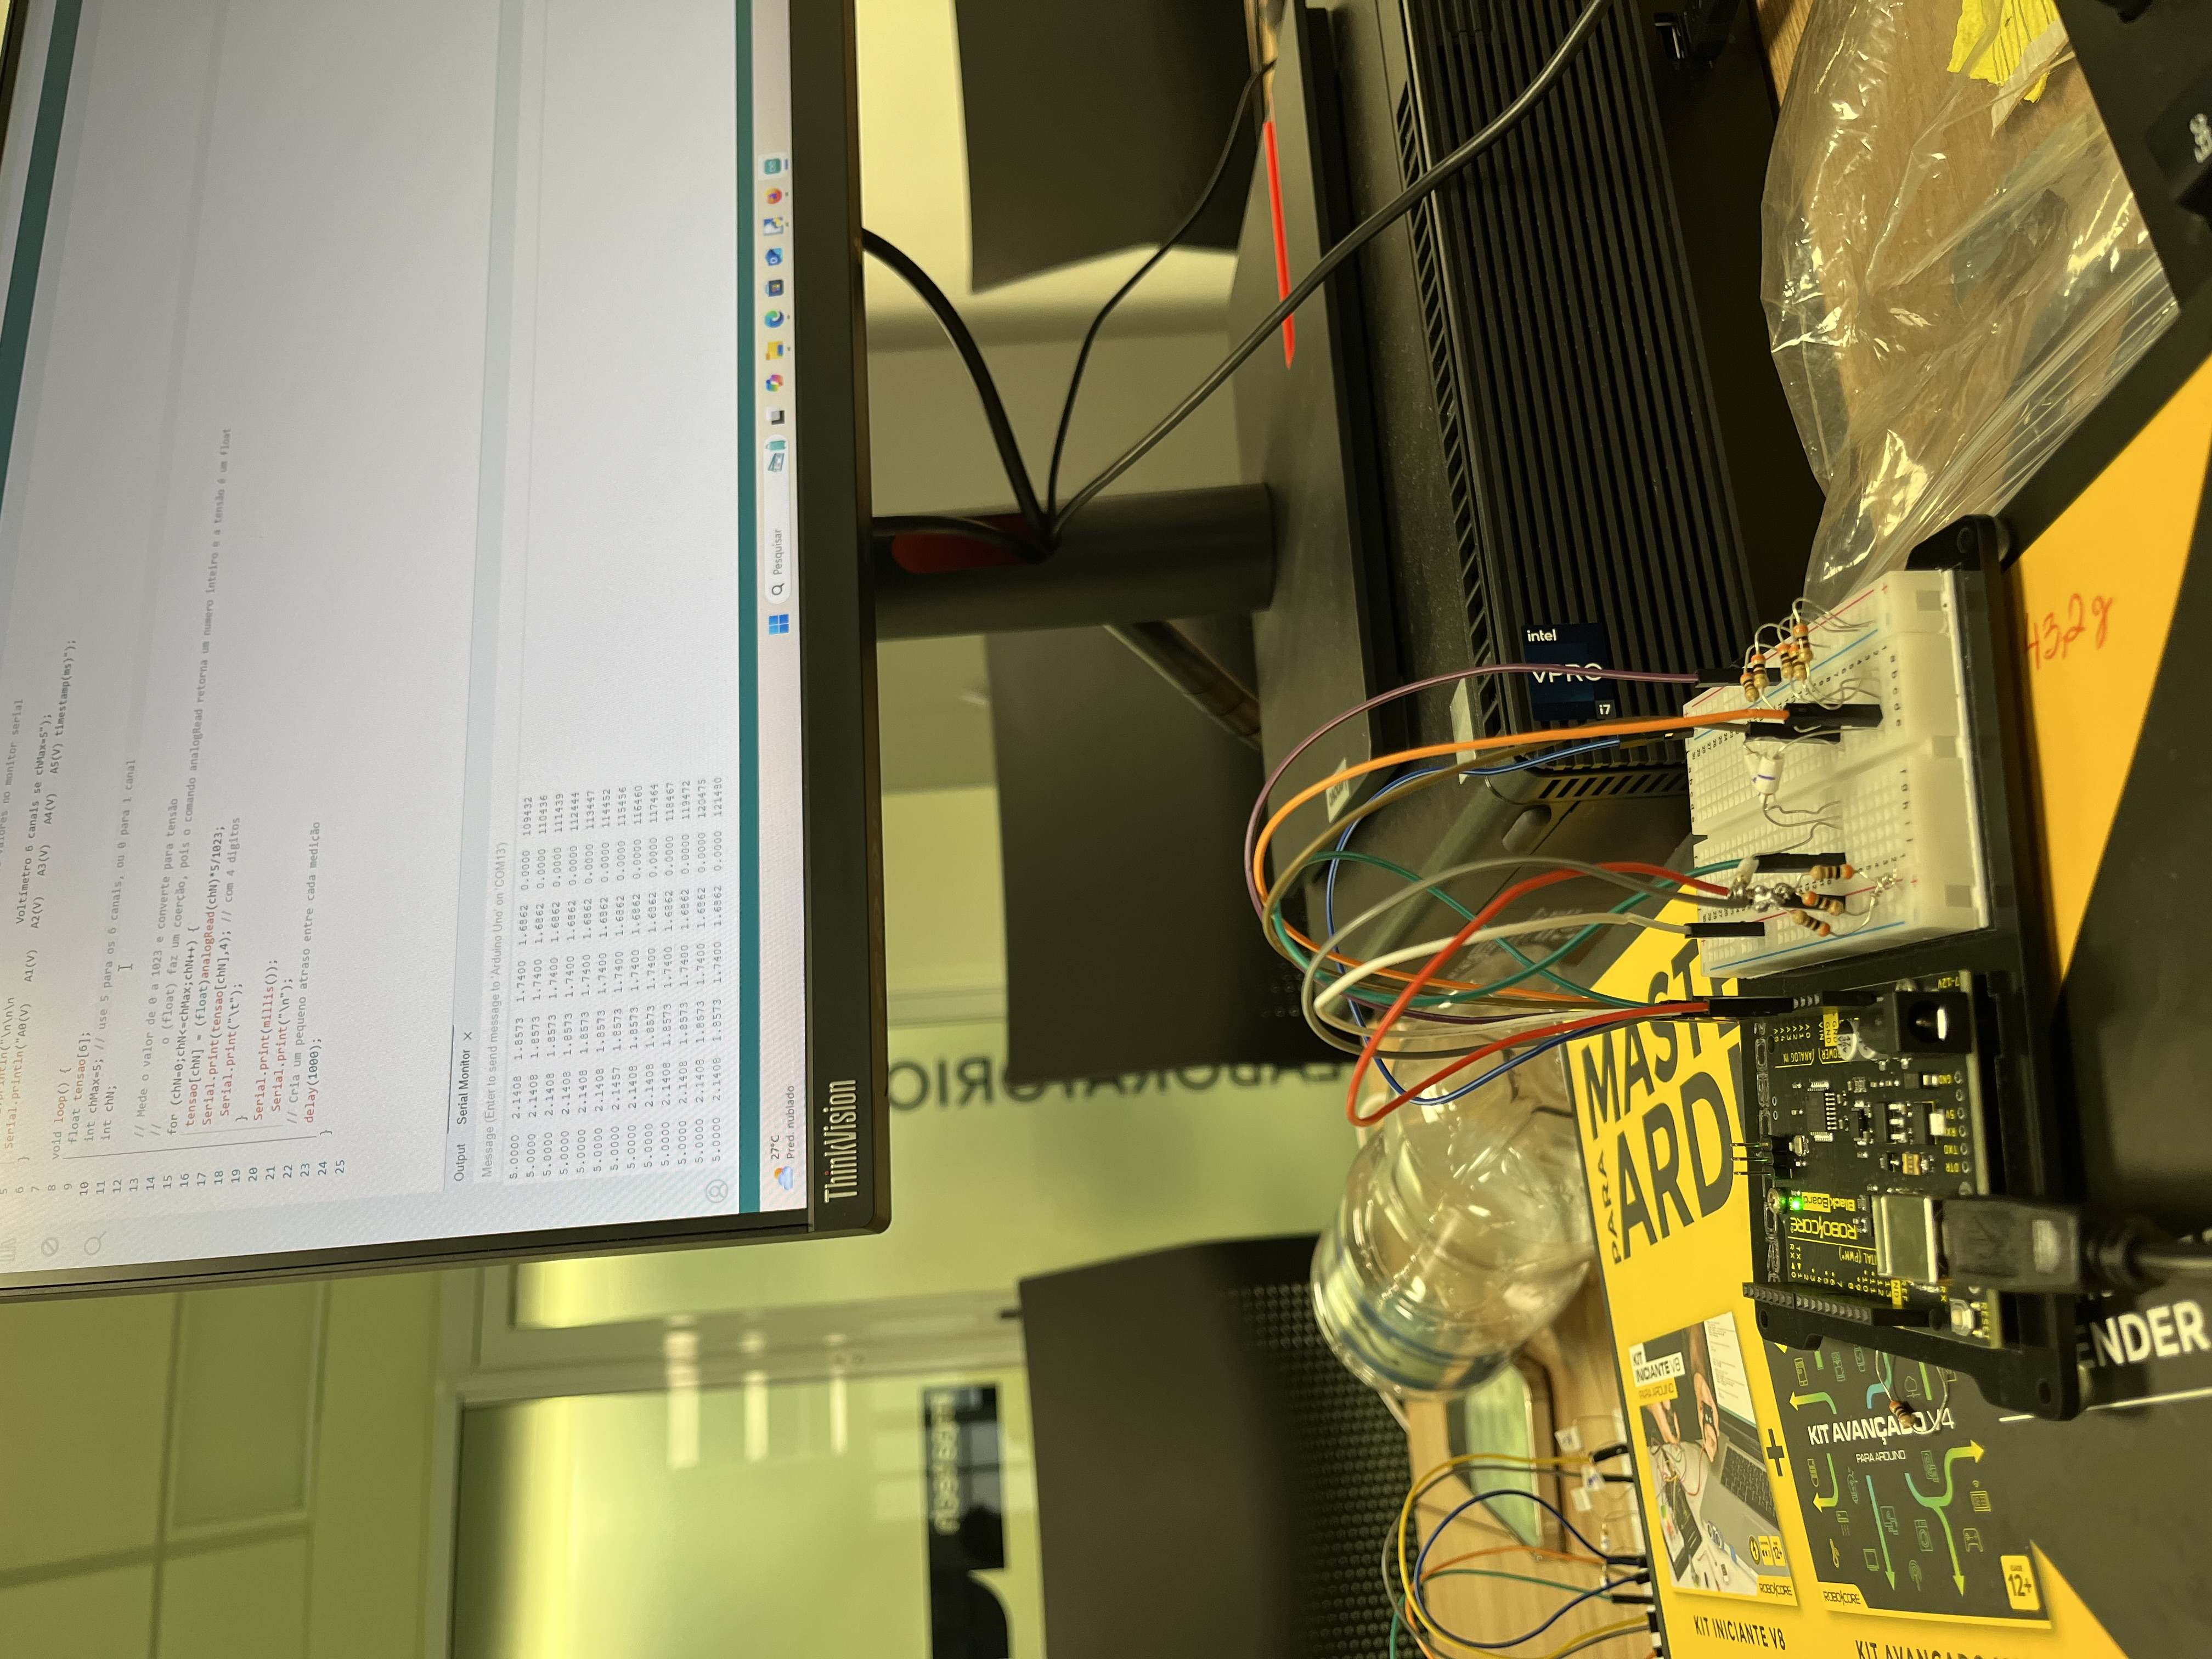
\includegraphics[width=0.8\textwidth]{IMG_3621.jpg} % Substitua pelo nome do arquivo da imagem
    \caption{Circuito montado no Arduino Uno.}
    \label{fig:arduino}
\end{figure}

\vspace{1em}

\subsection{Resultados}

\subsubsection{Dados}
\leavevmode

Depois de toda a simulação e a realização do experimento no Arduino Uno, obtivemos os seguintes valores das tensões:

\vspace{1em}

\begin{figure}[H]
    \centering
    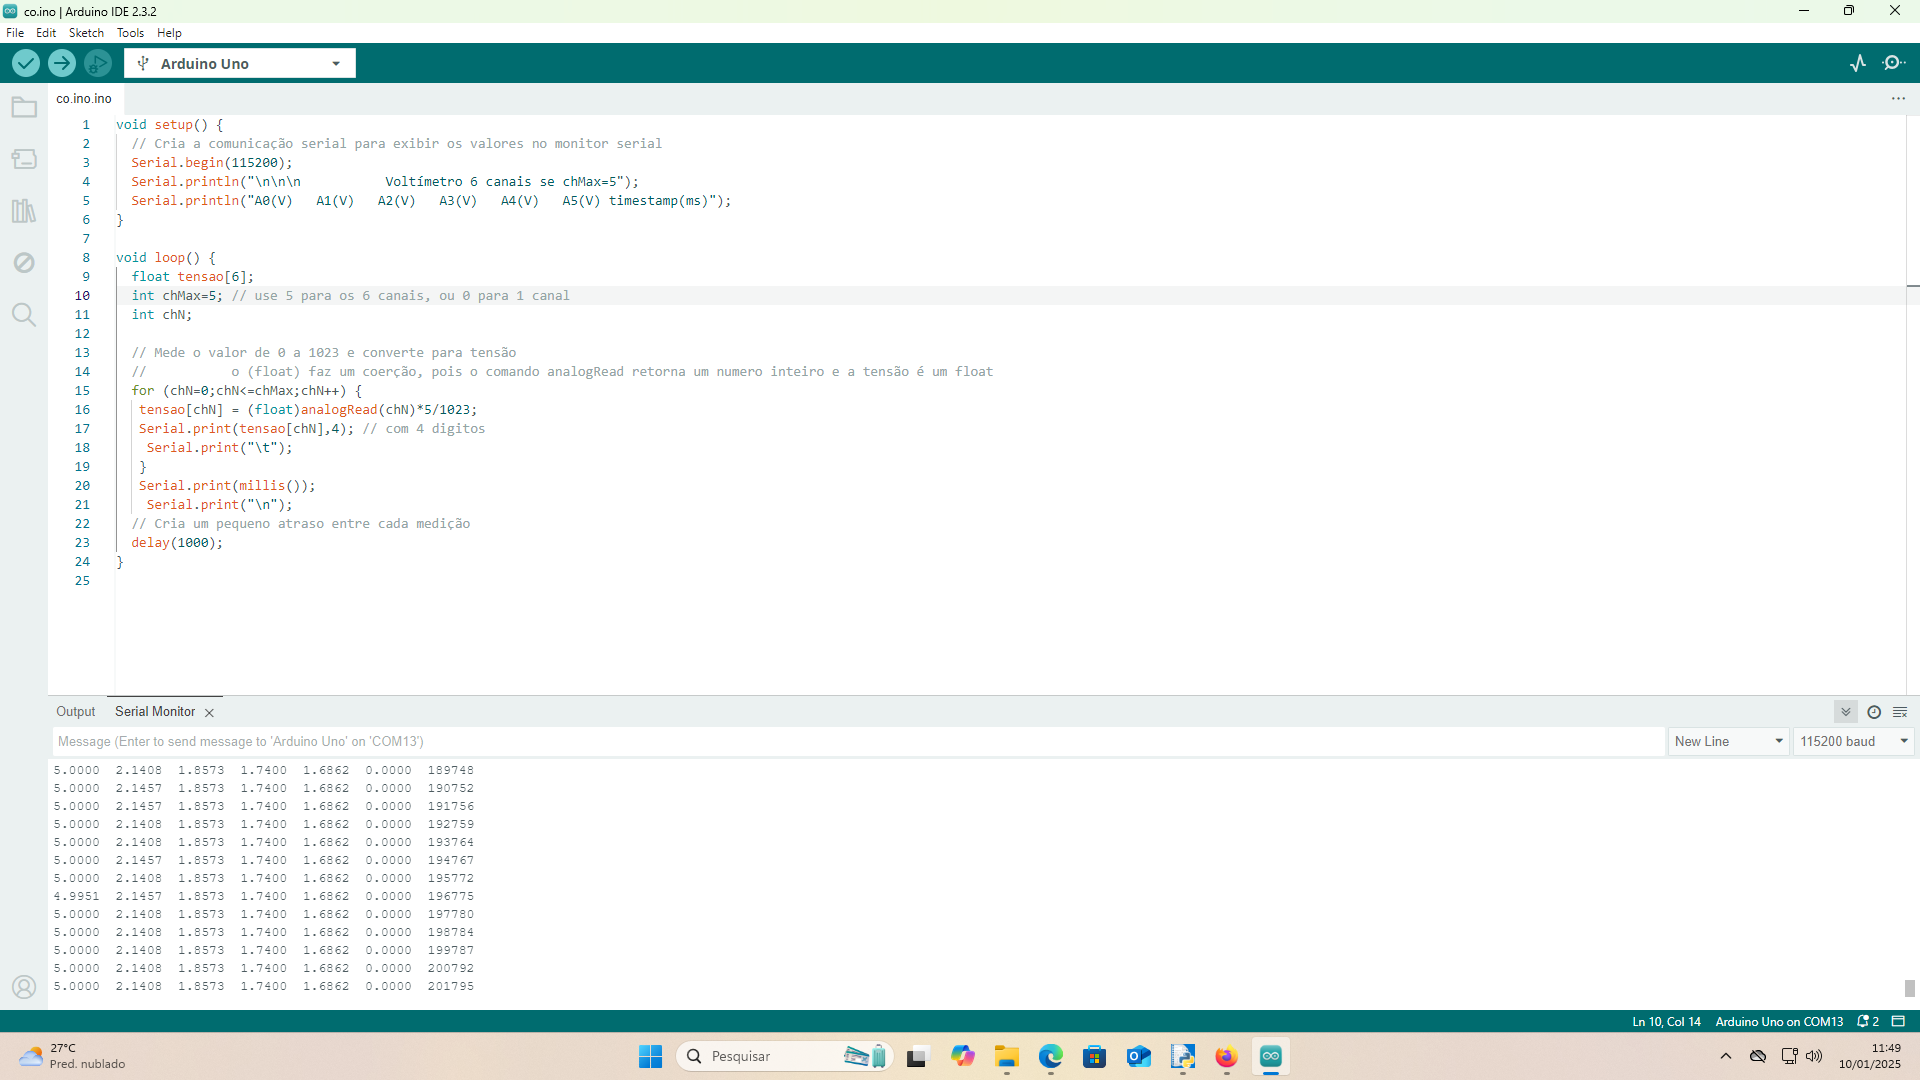
\includegraphics[width=0.8\textwidth]{Dados_exp03.png} % Substitua pelo nome do arquivo da imagem
    \caption{Tensões Obtidas}
    \label{fig:arduino}
\end{figure}

\vspace{1em}

\subsubsection{Análise}
\leavevmode

\subsection{Conclusão}
\leavevmode

\section{Referências}
\leavevmode

\end{document}
